\documentclass{article}
\renewcommand{\baselinestretch}{2} 

\usepackage[english]{babel}
\usepackage[letterpaper,top=2cm,bottom=2cm,left=3cm,right=3cm,marginparwidth=1.75cm]{geometry}

%Table Libraries
\usepackage{fancyhdr}
\usepackage[section]{placeins}
\usepackage{lscape}
\usepackage[table,xcdraw]{xcolor}
\usepackage{xurl}
\usepackage{graphicx}

%Header and Footer Settings
\pagestyle{fancy}
\fancyhf{}
\rhead{Jasmin Martin}
\lhead{21918141}
\usepackage{lastpage}
\rfoot{\thepage\ of \pageref{LastPage}}

% Useful packages
\usepackage{tikz}
\def\checkmark{\tikz\fill[scale=0.4](0,.35) -- (.25,0) -- (1,.7) -- (.25,.15) -- cycle;} 

\usepackage{amsmath}
\usepackage{graphicx}
\usepackage[colorlinks=true, allcolors=blue]{hyperref}
\graphicspath{ {./images/} }


\title{Synoptic Project Final Report}	% Title
\author{21918141}		% Author
\date{\today}			% Date

\graphicspath{{img/}}

%% Make title, author and date available via macros 
\makeatletter
\let\thetitle\@title
\let\theauthor\@author
\let\thedate\@date
\makeatother

\begin{document}
\begin{titlepage}
  \centering
  \vspace*{0.5 cm}
  
\includegraphics[scale = 0.15]{images/bucks-logo.jpeg}\\[1.0 cm]	   % University Logo
  \textsc{\LARGE Buckinghamshire New University}\\[2.0 cm]	   % University Name
  \textsc{\Large CO698WBL }\\[0.5 cm] % Course Code
  \textsc{\large BSc. (Hons) Digital and Technology Solutions Professional}\\[0.5 cm]			% Course Name
  \rule{\linewidth}{0.2 mm} \\[0.4 cm]
       { \huge \bfseries \thetitle}\\
       \rule{\linewidth}{0.2 mm} \\[1.5 cm]

       \begin{minipage}{0.4\textwidth}
	 \begin{flushleft} \large
	   \emph{Author:}\\
           Jasmin Martin (21918141)    % Author
	 \end{flushleft}
       \end{minipage}~
       \begin{minipage}{0.4\textwidth}
	 \begin{flushright} \large
	   \emph{Supervisor:} \\
           Jon Jackson     % Marker
	 \end{flushright}
       \end{minipage}\\[2 cm] 

       {\large \thedate}\\[2 cm]

       \vfill

\end{titlepage}

\newpage

\section*{Project Title}
\addcontentsline{toc}{section}{Project Title}
The research, design and development of a browser application, utilising natural language processing techniques, that can improve documentation comprehension by translating hierarchical file systems into visual interactive graphs

\newpage

\section*{Acknowledgements}
\addcontentsline{toc}{section}{Acknowledgements}
This dissertation has been completed as part of the New Buckinghamshire University Digital Technology Solutions Professional Apprenticeship scheme.

I would like to thank my supervisor Jon Jackson for his continuous support throughout the development of the project. His guidance and positivity was invaluable.

I would also like to extend my appreciation to my employer, Sky Ltd., and my colleagues for providing me with the opportunity to improve my technical skills. I hope to use my lessons from the project back in the workplace.

\newpage

\section*{Abstract}
\addcontentsline{toc}{section}{Abstract}
Computer file systems limit users to the hierarchical structure that can obscure related documentation located within different folders. Here, the author reports the development of a browser application which can convert a file system into a visual interactive graph that links documents by keywords. The application, called Atlas, uses natural language processing techniques to parse documents and generate graphical structures that demonstrate the relationships between documents. The author utilised the Scrumban agile methodology to iteratively develop the application by incorporating user feedback gathered from a series of presentations, surveys and interviews with members of their organisation. By engaging in each part of the product life cycle, the author was able to design, develop and deploy Atlas over the course of the synoptic project. Atlas can now be used to improve the comprehension of documentation, and in turn, increase the productivity of employees.

\newpage

\tableofcontents

\newpage

\section{Introduction and Background}

The aim of the synoptic project was to create an application that can identify and display links between documentation in a visual graph. The author designed and developed Atlas; a browser application that can convert a hierarchical file system into an interactive graph of documentation - termed the Atlas web. Each document was displayed as a single node in the Atlas web. Documents were linked to each other by common keywords (Figure 1). The purpose of Atlas was to clearly display the contextual information required for users to understand the relationships between documents and the underlying concepts they represented. Therefore, Atlas could increase the productivity of its users as the links promoted understanding and identified opportunities for collaboration between authors. 

\begin{figure}[!htb]
  \centering
      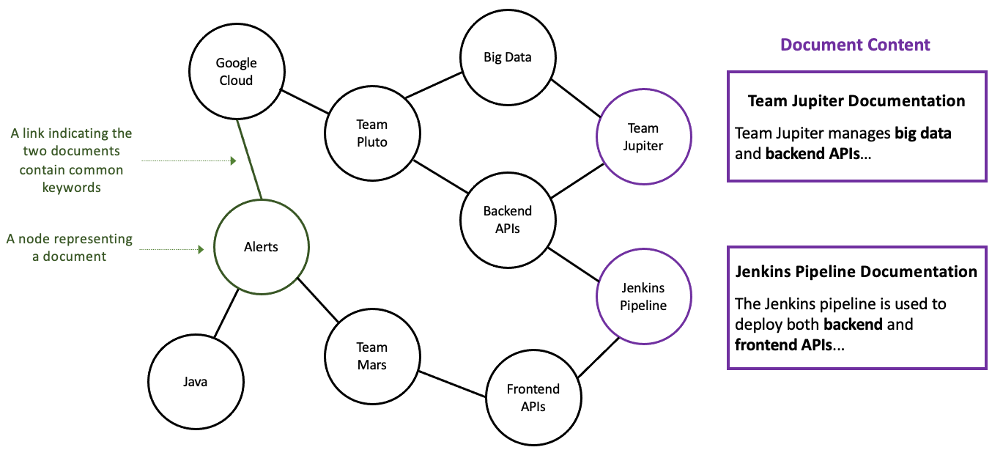
\includegraphics[width=1\textwidth]{images/web-intro.png}
  \caption{The Atlas web consists of document nodes that are linked by common keywords.}
\end{figure}


The idea behind Atlas originated from the author's struggle with understanding their department structure when they joined their current organisation. The hierarchical file system of documentation was disorganized, which in turn, made it difficult to navigate and hindered their ability to collaborate with others. Disorganized and outdated information within file systems is a common problem for large organisations, a study reported 73\% of new employees believed disorganisation within file systems reduced their ability to build relationships within companies (Rana et al., 2020). External knowledge management tools such as Roam an Notion have attempted to alleviate these issue by providing platforms that represented file systems as graphs. The key purpose of this project was to create a internal tool for generating graphs which would be cheaper and more secure that external solutions.

Atlas was designed and developed as part of the authors Digital and Technology Apprenticeship. The author furthered their professional skills by collaborating with colleagues to produce a solution that can improve the documentation structure for new employees in the department. The author improved their project management and technical abilities by engaging in the whole product life cycle from design, to development and deployment. In particular, the author learnt how to implement appropriate natural language processing techniques to process the large amounts of data within file systems. In this report the author describes the process of creating Atlas and links to the GitHub repository containing the software artefact. 


\newpage

\section{Strategic Rationale and Business Case}

\subsection{Benefits to Business}
The potential user base for Atlas was inherently wide, as file systems are common to nearly all computers. However, the author envisioned Atlas to be particularly beneficial to large organisations with complex organisational structures. Larger organisations are more likely to have more complex file systems, which in turn, have a greater change of becoming disorganised. Here, Atlas could be particularly useful as the Atlas Web could visualise the contextual links between documents which could reflect the relationships between ideas and teams.

The Atlas Web is more valuable than even the most organised hierarchical file systems, as the user is not limited within the context of a folder (Figure 2). Instead, their scope is broadened as they are able to see an overview of all documents. The Atlas Web was designed to improve the productivity and efficiency of users, as they are able to easily understand the relationships between concepts, with some links providing the opportunity for collaboration. Furthermore, duplicated or disorganised documentation can easily be identified within the Atlas Web (Figure 3). Resulting clarifications could lead to less duplicated work in the business and more knowledge sharing.

\begin{figure}[!htb]
  \centering
      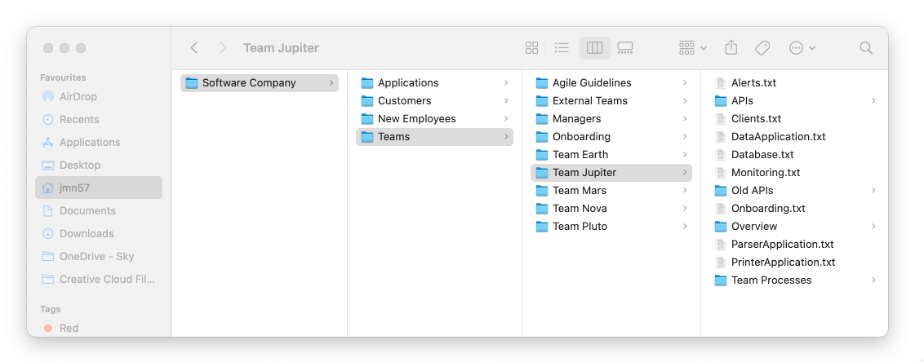
\includegraphics[width=1\textwidth]{images/filesystem-business-case.png}
  \caption{The traditional hierarchical file system limits users within the scope of folders.}
\end{figure}

\begin{figure}[!htb]
  \centering
      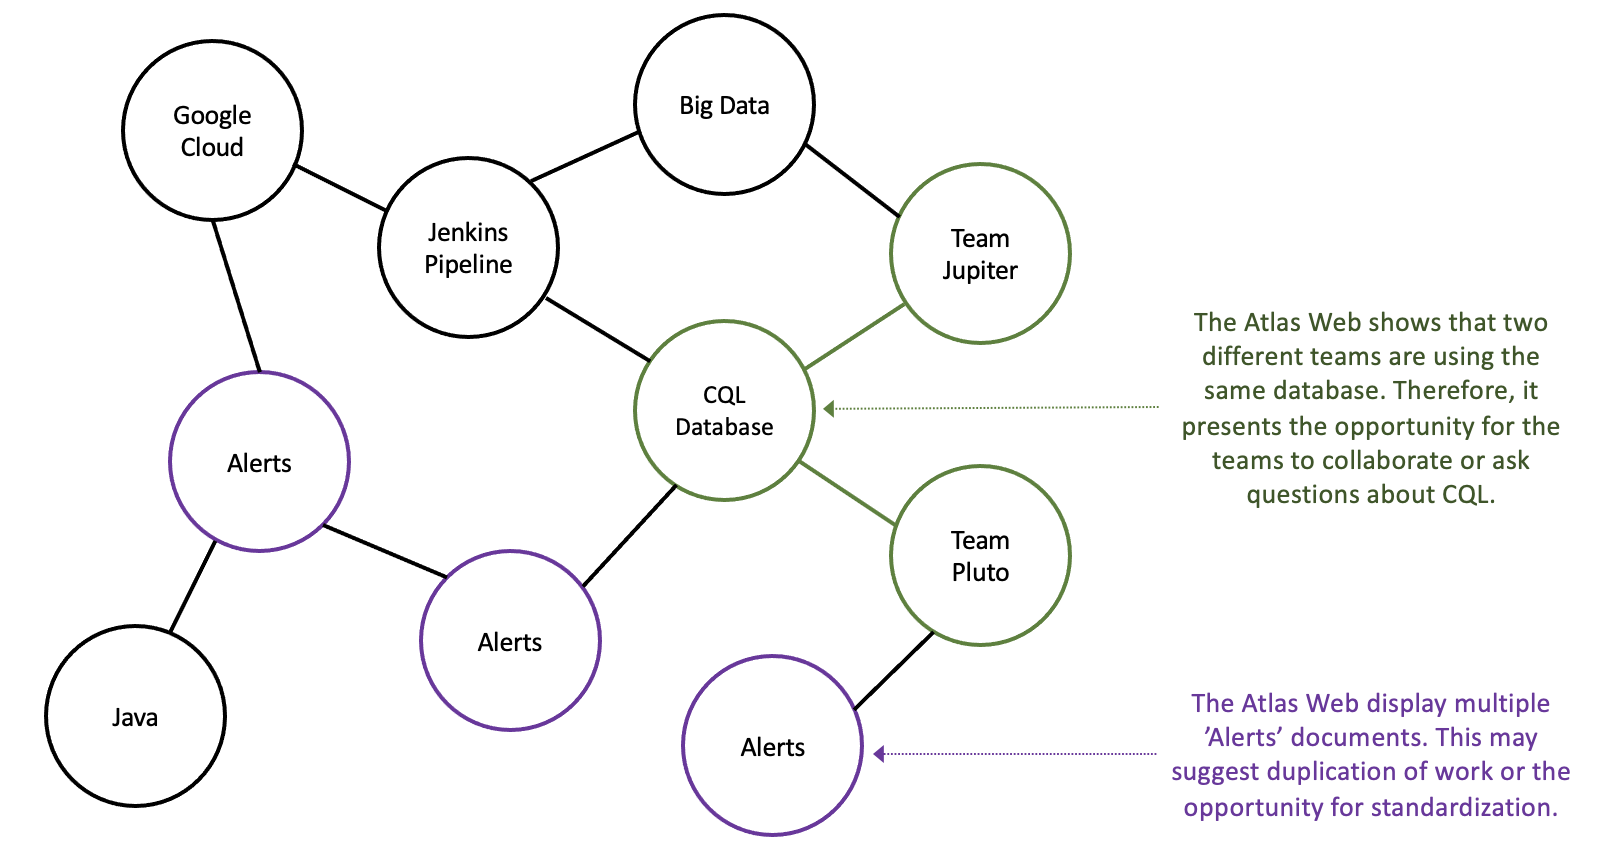
\includegraphics[width=1\textwidth]{images/benefits-of-web.png}
  \caption{The Atlas Web creates the opportunity for teams to collaborate and share knowledge.}
\end{figure}

It is important to recognise that the effectiveness of tools like Atlas is not anecdotal, rather the benefits have a scientific basis. Research has shown visual devices such as mind-maps and diagrams similar to those generated by Atlas are more effective at conveying information than text-based structures (Johnson-Laird, 1983). This preference for visual information has been proven in multiple contexts. For instance, when learning to read, children respond faster when presented with word and picture combinations, than the written words alone. Although this preference for visual word pairs fades with age, the increased comprehension of diagrammatically displayed information remains in adulthood (Coleman et al., 2018). This was confirmed by a study that revealed students taught with integrated text diagrams performed better on tests as opposed to students who were presented with text (Hegarty et al., 1991). 

Visual aids are particularly useful when representing complicated events, concepts, or relationships which would otherwise be difficult to portray with words. Although the degree of comprehension of a visual aid will increase with the individuals' cognitive aptitude and profile, generally, the presence of visual aids enables individuals to coordinate both the information from the text and the diagram to create more meaningful linkages (Schieter and Eitel, 2015). This research supports the basis that Atlas could increase the overall comprehension of documentation. A large organisation, such as the authors employer, with complex documentation could benefit from having a more visual way of conveying information. In particular, Atlas could become effective for new employees whom could utilise the Atlas Web to familiarise themselves with the organisational structure. Research suggests that employees may not become effective in their role until they have a good understanding of the organisation structure (Dohetry et al., 2010). Therefore, Atlas could become paramount in reducing the time taken and financial cost of on boarding. 

\subsection{Survey of Competing Products}

Before developing Atlas, the author analysed several competing software solutions to determine whether a knowledge management tool should be purchased rather than developed in house. Several similar software applications offer a solutions to documentation visualisation. The most popular of which is Roam. Roam has been described as a “note-taking application for networked thought” (Roam, 2021) (Figure 3A). Like Atlas, Roam links documents by keywords to produce a visual overview of all documentation. Roam gained popularity as an early visual note taking tool and was recently valued at \$200 million. Roam is used by clients such as CodeAcademy, CapgeMini and Match to support and share their large documentation structures with employees (Clark, 2020). In contrast to Roam, Obsidian is a newer freely available tool, with similar documentation web generating functionality (Figure 3B). Obsidian is not hosted on a website, rather it requires users to download and use the tool locally (Obsidian, 2021).

\begin{figure}[!htb]
  \centering
      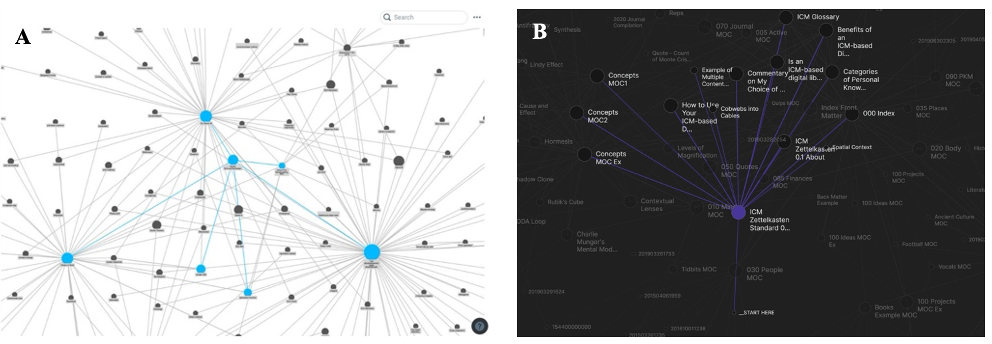
\includegraphics[width=1\textwidth]{images/roam-and-obsidian.png}
  \caption{The web interfaces of competing software applications offering visual based document structures; Roam (A) and Obsidian (B).}
\end{figure}

Although, current documentation visualisation tools offer a similar functionality as Atlas, developing an in house tool would be more beneficial to the authors organisation as it would be cheaper, more secure and extensible. Roam operates on a subscription based financial model. For organisation with less than 500 members, Roam can cost up to \$8 per user (Roam, 2021). Cheaper solutions such as Obsidian may be appropriate for smaller organisations, whose employees have a good technical knowledge. However, for an organisation with non-technical employees, it is unlikely the application would be utilised as it required the ability to effectively use command-line base tools. The market for freely available knowledge management tools is limited by their ability to succinctly display large quantities of documentation to non-technical users.

The development of Atlas was completed by a single developer, on one day per week, over the period of several months. As Atlas was developed as part of an apprenticeship degree, there was no immediate cost incurred to the authors organisation. However, after this initial development period, the further development and maintenance of Atlas would require further funding. These costs were anticipated to be relatively low as the application was planned to be functionally complete by the end of the development period. As the application did not rely upon any external feeds for live data, it would require minimal support. The hosting cost of the application would be relatively low, as the organisation had already negotiated a corporate contract which would accommodate the deployment of applications such as Atlas. Any further feature of bug development could be weighed against the uptake of the application in the company and the benefits it could bring. 

\subsection{Benefits to Author}

The intention of Atlas was not only to create a useful product for the organisation, but to also demonstrate and improve the author's software skills. Atlas presented the opportunity to develop and manage a greenfield project. This exercised the authors project organisation skills and technical abilities. The project enabled the author to demonstrate their skills to their current employer. Furthermore, as other employees were consulted for the project, it enabled the author to build more relationships within organisation.

\newpage

\section{Ethical Considerations}

All software application must respect the privacy of their users. On the development of software, it is vital to ensure permissions are obtained, identities are obscured and confidentiality is maintained (Winter, 1995). When consumer research was conducted for Atlas, the author ensured that all partakers in the research were aware of the intentions of the project. To ensure the confidentiality of those who engaged in any research or testing of Atlas, no person was named in the report. As both the project and report were independent of others’ work, no descriptions of other projects were negotiated with any other person. 

As Atlas parsed user inputted files, it was important to ensure that the content was secure. Atlas did not utilise a database, rather the application was compiled locally and files were stored in memory on the users machine. Therefore there was no concern for the safety of the data as it could not be accessed by external parties.

All libraries utilised by Atlas were open source and did not require licenses. A list of them can be found in the Atlas GitHub repository.

The ethical checklist required for the synoptic project can be found in Appendix B.

\newpage

\section{Aim and Objectives}

\subsection{Project Aim}

The aim of the synoptic project was to create a browser application that could convert a file system into a visual interactive graph that links documents by keywords. The graph, known as an Atlas Web, would clearly demonstrate to the user the relationships between different documents. As a result, the application would promote more collaborative and creative processes. Atlas would improve the documentation comprehension within the authors company as it currently has a high number of complex file systems which are currently difficult to depict without diagrams. The author aims to design, develop and test the greenfield product within their organisation to create a software solution which benefits their colleagues and enables the author to improve both their technical and management skills.

\subsection{Project Objectives}

The author outlined four objectives at the start of the synoptic project that encompassed the product design, development and deployment.

O1. Design a user interface that clearly depicts the relationships between different documents.

O2. Develop a minimal viable product that can generate an Atlas Web from a local file system.

O3. Gather and incorporate user feedback on the minimal viable product to develop improved iterations of the application that contain requested features.

O4. Deploy the product and make the code open source. 

\newpage
\begin{landscape}
\thispagestyle{empty}

\section{Risk Management}
  \centering
      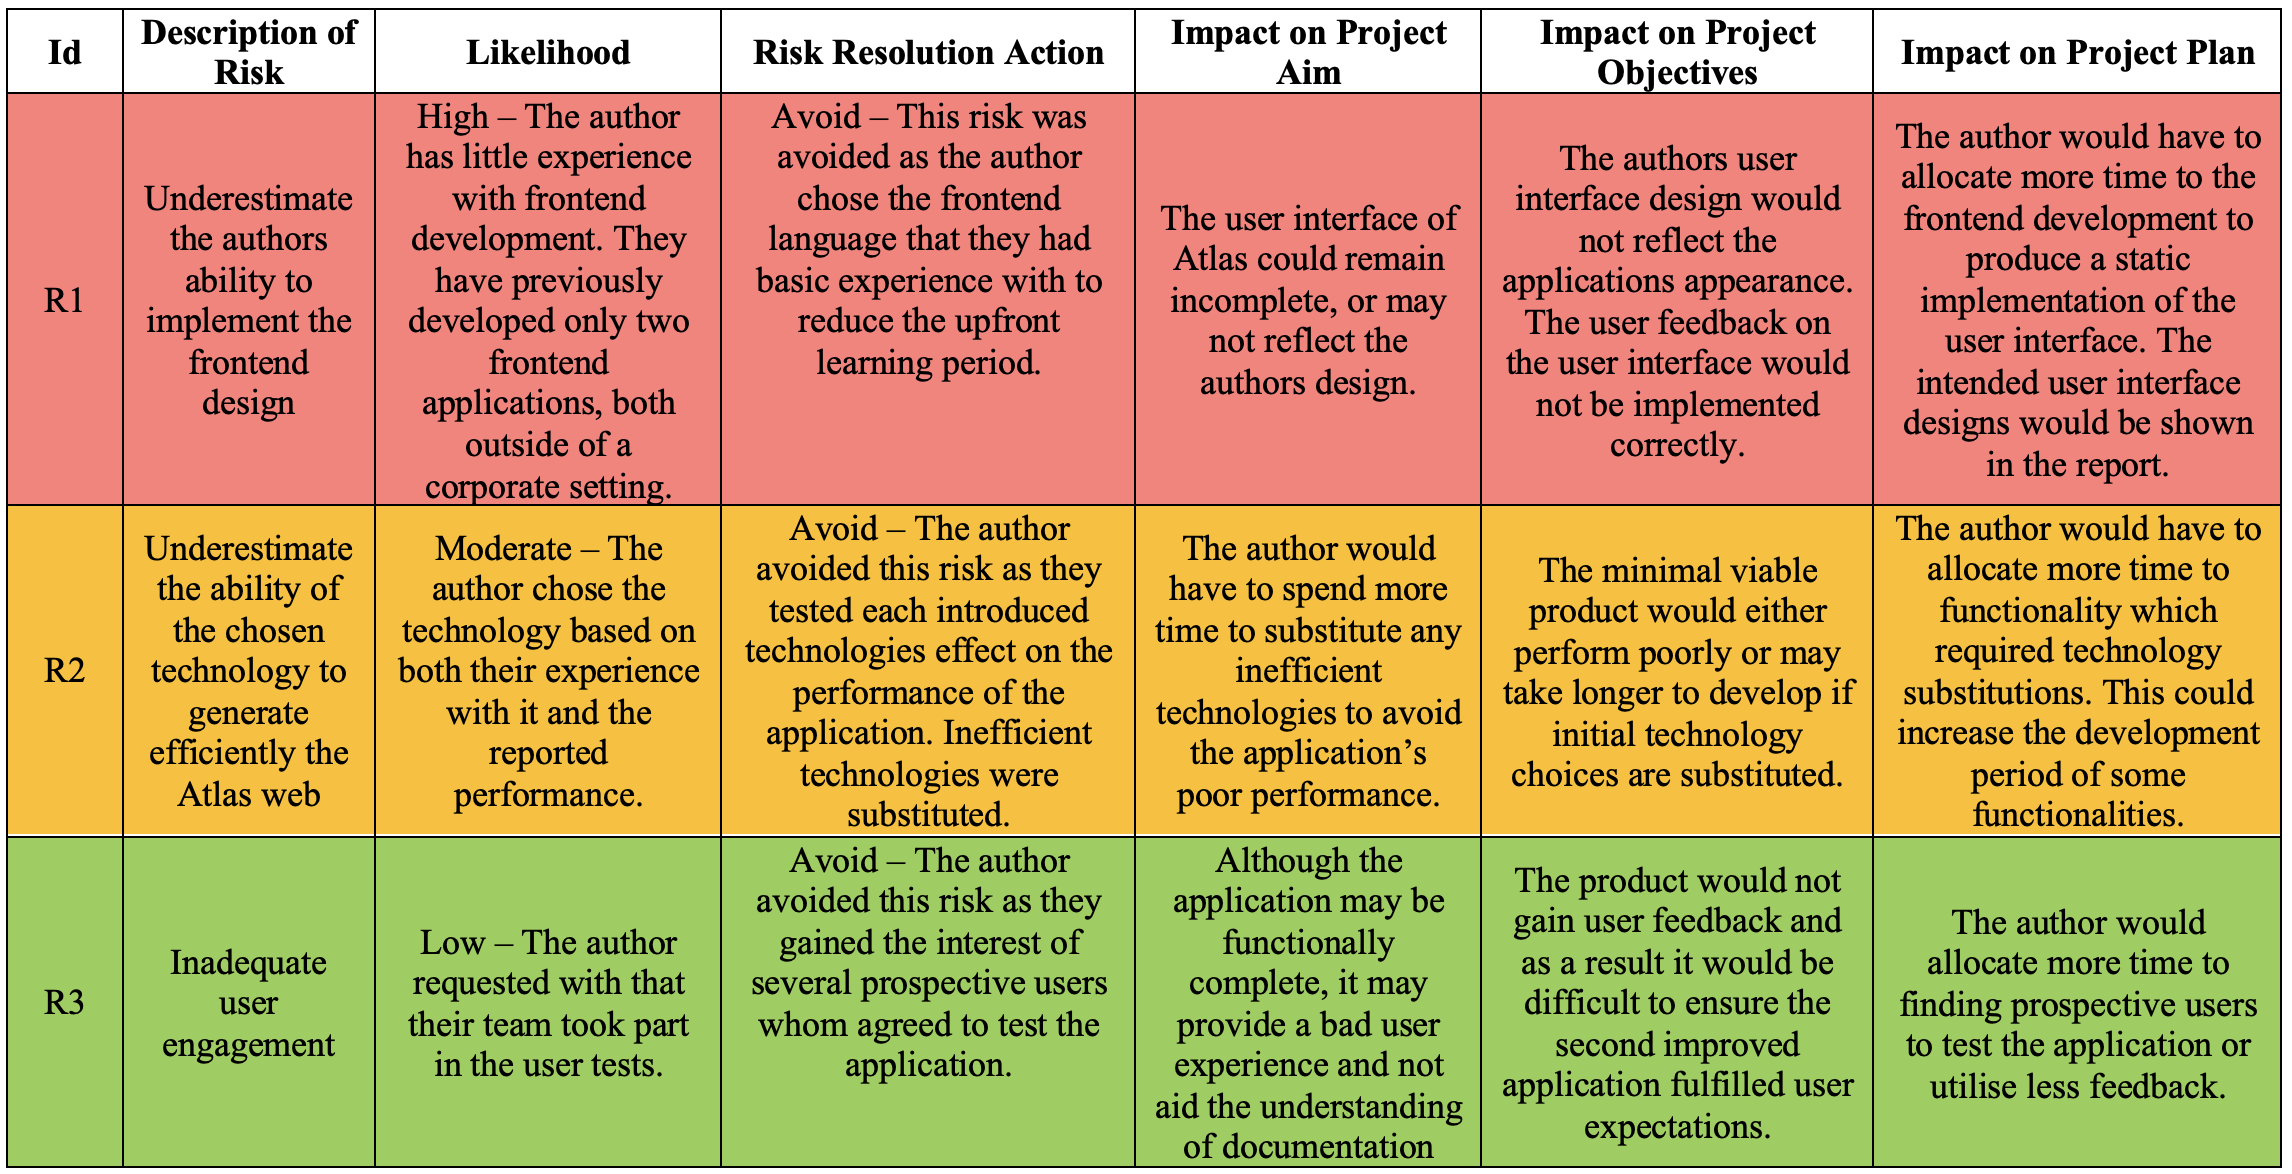
\includegraphics[height=12cm]{images/risk1.png}
\vfill
\raisebox{0.2cm}{\makebox[\linewidth]{Page \thepage}}

\newpage
\thispagestyle{empty}
  \centering

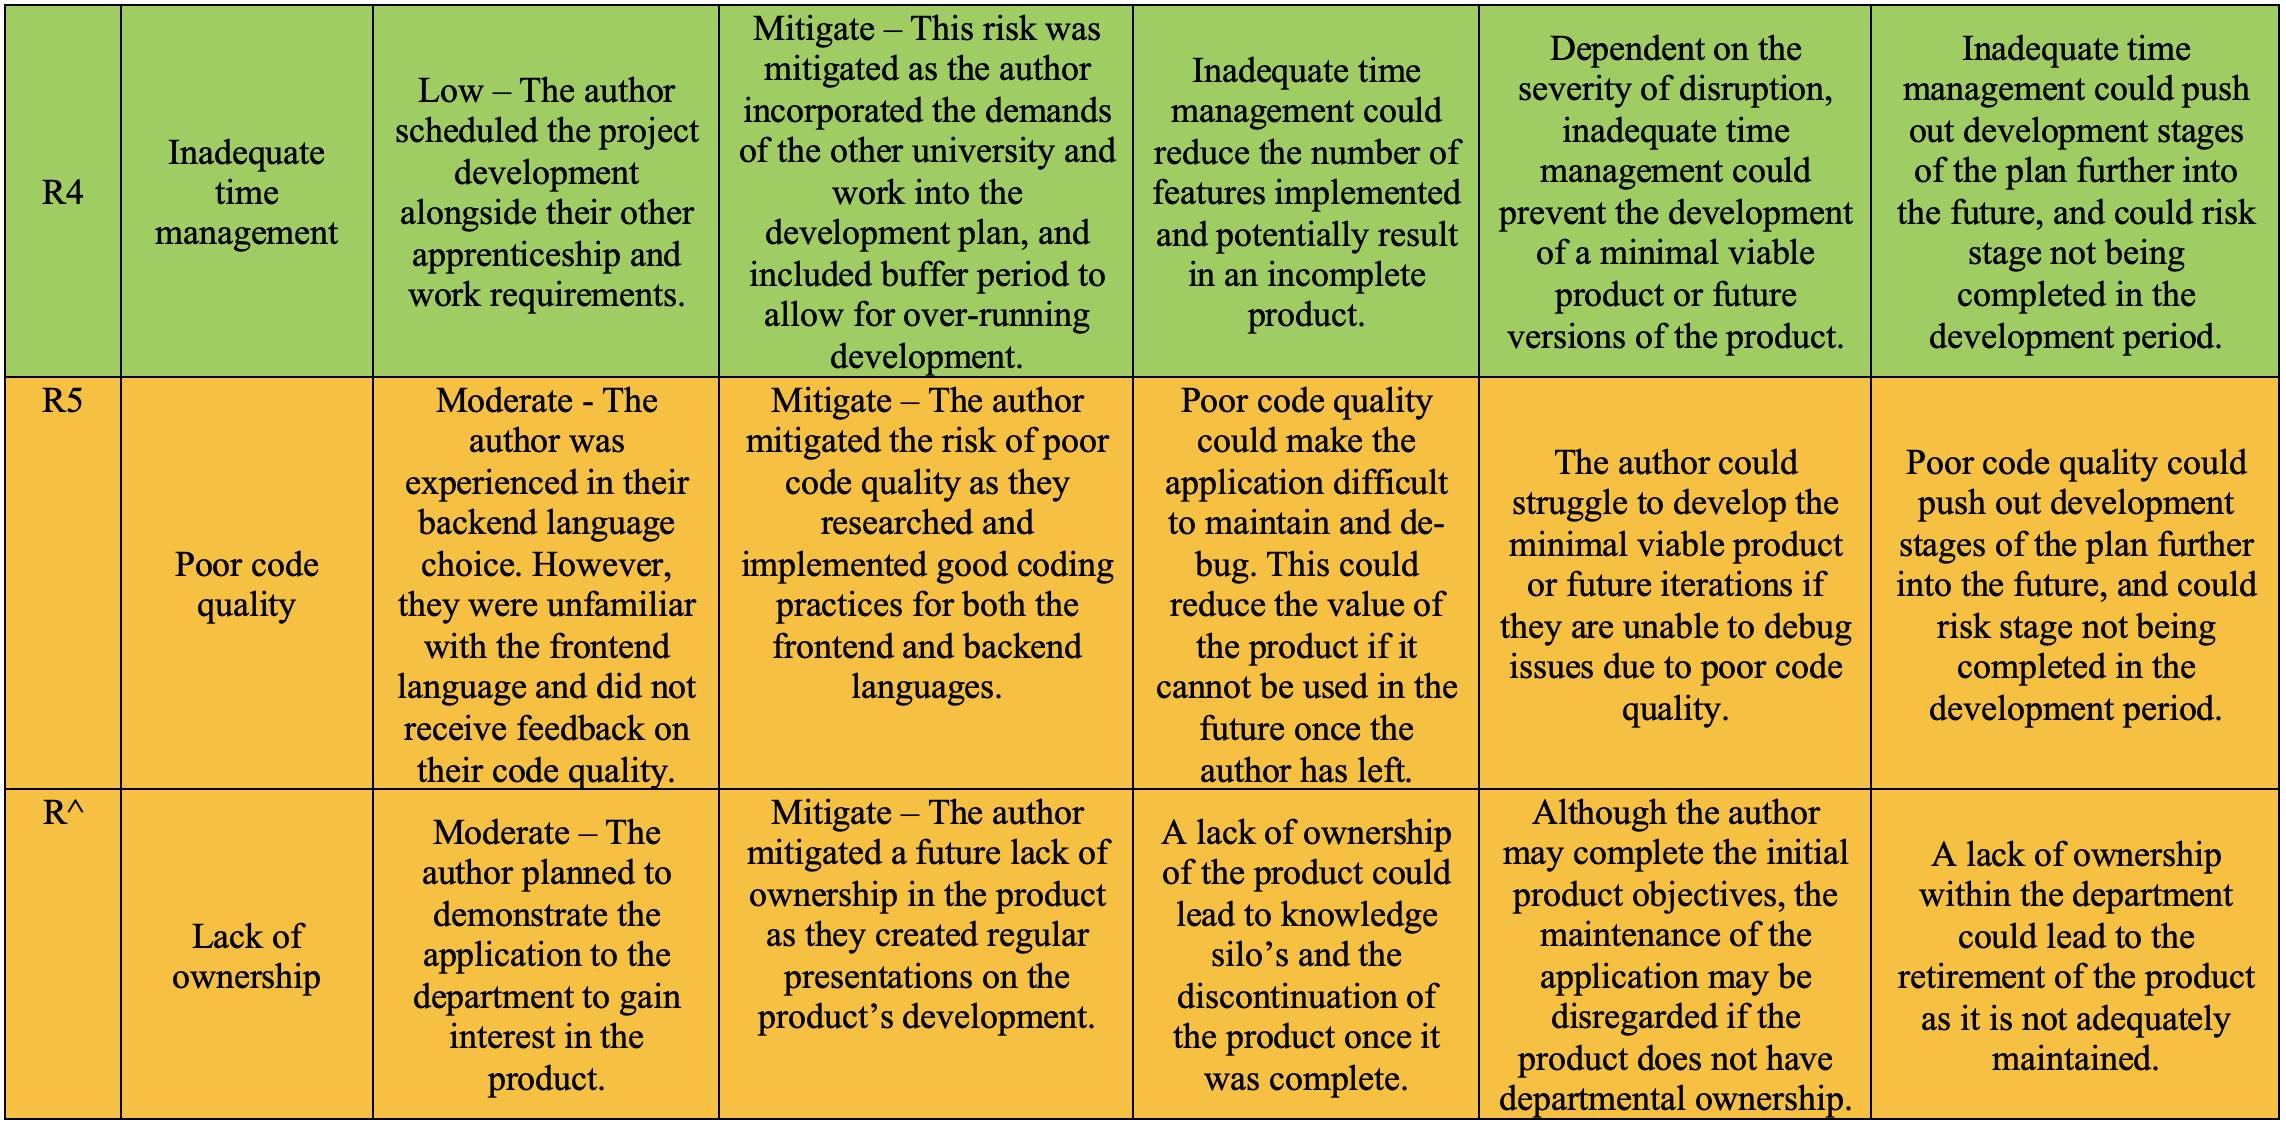
\includegraphics[height=12cm]{images/risk2.png}

\vfill
\raisebox{0.2cm}{\makebox[\linewidth]{Page \thepage}}
\end{landscape}

\newpage

\section{Literature Survey}

In this literature review the author explored the theory, technology and project management techniques that were used in the design and development of Atlas. In order to meet the outlined aims and objectives, the author explored unfamiliar technical areas such as natural language processing and artificial intelligence. To ensure the appropriate project management style was selected, the author reviewed popular management styles and selected the appropriate method.

\subsection{The Algorithm Behind Atlas}

The underlying algorithm that connects related documents in the Atlas Web is known as the Zettelkasten method. The Zettelkasten method was developed by Niklas Luhmann (1927 – 1998) (Ahrens, 2017). Luhmann was a prolific sociologist who championed neither the short and long-term memory of the human brain could comprehend large quantities of data (Ludecke, 2015). To develop a more intelligible solution to storing and organising notes, he developed the ‘slip-box’ (or Zettelkasten in German). The Zettelkasten method states a single index card that contains one idea, which would be singularly referenced by a sequential number (i.e 1). If a new note was to be made with the same theme, Luhmann then added a new index card and appended the reference with a letter (i.e. 1a.). Then, if another noted related to the branched index card, it would then be similarly be referenced to (e.g. 1b) (Figure 5). The output of the Zettelkasten method is a database of index cards that can be extended indefinitely in any direction as each index card pertained to a static reference (Forte, 2020). 

\begin{figure}[!htb]
  \centering
      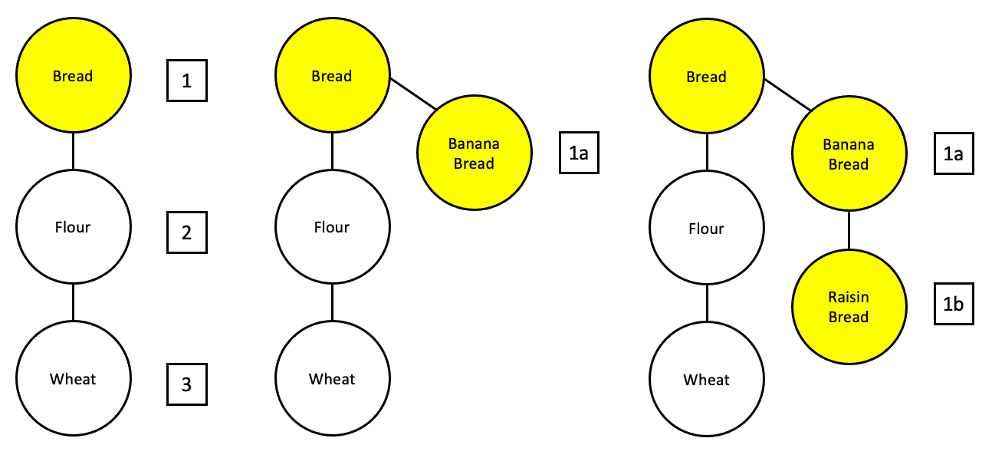
\includegraphics[width=1\textwidth]{images/litreview-zettelkasten.png}
  \caption{Niklas Luhmann’s Zettelkasten method enables users to create a database of notes, linked by topic. This is the algorithm used by Atlas.}
\end{figure}

The  Zettelkasten method produces a fluid but organised network of notes. The relationships between notes are clearly displayed, making each note more valuable as ideas are organised into reusable and reflective threads (Gibson, Gregory, and Robson, 2005). The graph of relationships provides a clear external basis of existing knowledge which compliments a more natural thought process as users can focus on elaborating ideas (Gibson, 2020). In turn, this can increase productivity as knowledge is gained more quickly and users can make more informed decisions (Glaser and Strauss, 1967). Furthermore, displaying the whole system of notes provides the opportunity for accidentally encountering links between subjects that hadn’t been anticipated. The key benefit of creating an application that uses this algorithm is that the referencing is automated. Instead of storing and searching for physical cards to reveal information, Atlas will display the relationship to the user clearly and instantly.

A potential criticism of the Zettelkasten method is that the user may find that they are creating ideas that are contradictory or paradoxical. For instance, a user may find that two notes exist, with differing information. However, it could be argued that this is not a limitation of the Zettelkasten method, rather it is a feature. The Zettelkasten method brings these contradictions to light, adding ideas to a discussion. Contradictory data is valuable to discussions, as it represents a misalignment of knowledge and often opens new paths of inquiry (Forte, 2020). Furthermore, seeing different conclusions of the same ideas shares perspectives. By placing incompatible theories side by side, we encourage the skill of objectivity and stop users from jumping to conclusions. This independent thinking counteracts confirmation bias – our tendency to just believe information that we already know – and forces the user to confront misunderstandings (Gibson, Gregory and Robson, 2005). If Atlas was used in a large corporation, the revelation of contradictory or duplicated notes could lead to discussions or collaboration to align team and departmental knowledge.


\subsection{Project Management Techniques}

Software project management techniques are both the science and art of planning and directing software projects (Wasserman, 2010). To be effective, software project management techniques should account for the whole project life; from the initial product design, to the planning of tasks, effort estimation, work supervision, and the testing of the end product (Dyba, Dingsoyr and Moe, 2014). Such management practices have been developed with a culmination of years of trial and error. Although each technique may differ in practice, they all share the ultimate goal of building better software (Hoda, Noble, Marshall, 2008).

The agile development approach was used to develop Atlas. In agile development, developers work with end-users to implement functionality in iterative cycles. Rather than having a fixed plan,  developers respond to changing requirements in real-time (Stellman and Greene, 2008). This ethos reflects the principles outlined by the original Agile Manifesto (Fowler and Highsmith, 2000). The agile methodology opposes the traditional well-defined linear sequence of activities that traditional management techniques such as Waterfall define. Instead, the agile methodology recognises that activities may require a shorter time between planning and execution. As a result, planned features do not contains all the details of the implementation and are not planned far in advance (Hoda, Noble, Marshall, 2008). 

A particular offshoot of agile known as Scrumban was selected as appropriate project management technique for Atlas. Scrumban is an amalgamation of two popular agile practices; Scrum and Kanban (Table 1). Both practices promote the fundamental agile tenant of utilising iterative and incremental techniques to quickly gain feedback on development cycles. The Scrum process defines specific individual roles, work requirements and time boxes that define clear developmental goals. Kanban, on the other hand, offers a system for visualizing a continuous flow of work. Scrumban provides the structure of Scrum and flexibility and visualization of Kanban. 


\begin{table}[]
\caption{An overview of Scrum, Kanban and Scrumban development methodologies. Highlighted cells reflect the chosen management techniques. Content adapted from Arbaham, 2021.}

\centering
\resizebox{\textwidth}{!}{%
\begin{tabular}{|l|l|l|l|}
\hline
 & \textbf{Scrum} & \textbf{Kanban} & \textbf{Scrumban} \\ \hline
\textbf{Timebase} & \cellcolor[HTML]{92D050}1- 4 weeks & No time base & 3 month buckets \\ \hline
\textbf{Rules} & Constrained process & Flexible process & \cellcolor[HTML]{92D050}Slightly restricted process \\ \hline
\textbf{Roles} & \begin{tabular}[c]{@{}l@{}}Product owner, scrum master,\\  scrum team, stakeholder\end{tabular} & No specific roles required & \cellcolor[HTML]{92D050}No specific roles required \\ \hline
\textbf{Board} & Defined/resets each week & Persistent – the Kanban board & \cellcolor[HTML]{92D050}Persistent – the Scrumban board \\ \hline
\textbf{Prioritization} & \cellcolor[HTML]{92D050}Backlog & Optional & Recommend on each planning \\ \hline
\textbf{Estimation} & Before sprint starts & Optional & \cellcolor[HTML]{92D050}Optional \\ \hline
\textbf{Planning routine} & Sprint planning & On demand & \cellcolor[HTML]{92D050}On demand \\ \hline
\textbf{Performance metrics} & Burn down & Cumulative flow diagram & \cellcolor[HTML]{92D050}Average cycle time \\ \hline
\end{tabular}%
}
\end{table}

The development of Atlas was well suited to Scrumban as the project exhibited a high variability in requirements, skills, and technologies (Augustine et al., 2005). Therefore, Scrumban would provide a clear progression of the project tasks. Progression awareness was particularly important for Atlas as the project was developed intermittently by a single developer. The short development cycles, common to agile practices, enabled the user to quickly gain the user feedback that enabled the quick identification of problem areas and the subsequent prioritisation of features (Asra, Sobia, and Khan, 2014). 

The author deviated slightly from the pure Scrumban style, as they favoured two key Scrum aspects: a shorter iteration cycle of two weeks and the presence of a backlog. The smaller development cycles and backlog promoted more forward planning and helped the author remain organised. In addition to Scrum and Kanban, the author also took the Extreme Programming practice of utilising spikes. Spikes are time-boxed explorations into technologies or solutions (Jeffries, 2001). Spikes were appropriate for Atlas as the author was utilising weaker skills such as front-end development.

\subsection{Natural Language Processing}

In this project, the author researched natural language processing techniques. Natural language processing (NLP) is a sub-field of computer science that revolves around analysing, processing and representing human language (Damerau and Indurkhya, 2010). Researchers of natural language processing apply machine learning algorithms to speech and text to achieve human-like language processing (Chowdrhy, 2005). The application of NLP research includes predictive typing, speech recognition, and spam detection (Ventsislav, 2018).

The fundamental feature of Atlas is the ability to translate a hierarchical file system structure into the Atlas Web. To achieve this, all folders and documents in the file system must be scanned and keywords must be identified and stored. In the field of NLP, this process is known as deductive parsing (Trujillo, 2018). A deductive parsing algorithm has two distinct elements: a parser which will scan each word, and a tokenizer which will check for pre-defined tokens in the input (Chowdrhy, 2005). For Atlas, the keywords identified by the tokenizer were surrounded by square brackets (e.g. [[keyword]]).

In addition to parsing and tokenisation, Atlas would also be developed to utilise the natural language processing techniques, stemming and lemminisation. The goal of both stemming and lemmatization is to reduce inflectional forms of words in order to form a common base (Jivani, 2011). These processes would be integral to Atlas, as they would prevent multiple derivatives of the same word from being created. Understanding the subtle difference between these two processes was important in order to prioritise and implement the techniques (Figure 6). Stemming is the crude process of removing the end of words, in order to chop off derivational affixes (i.e. ‘run’ and ‘running’). Lemminisation is a more complex process that conducts a morphological analysis of words, removing inflectional suffixes to return the dictionary for a word known as a lemma (i.e. ‘study’ and ‘studies’) (Ventsislav, 2018). This research led the author to prioritise, implementation of stemming first, with the goal of implementing the more complex lemminisation for the end product.

\begin{figure}[!htb]
  \centering
      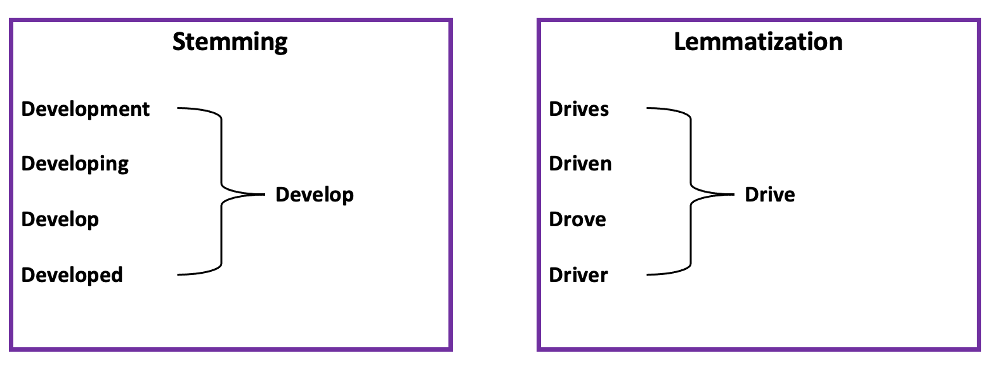
\includegraphics[width=1\textwidth]{images/litreview-nlp.png}
  \caption{Niklas Luhmann’s Zettelkasten method enables users to create a database of notes, linked by topic. This is the algorithm used by Atlas.}
\end{figure}

\subsection{Artificial Intelligence}

Atlas would incorporate elements of artificial intelligence as it would be able to recommend common keyword tags. Artificial intelligence enables machines to complete tasks that would require intelligence if completed by a human (Boden, 1997). A famous early example of artificial intelligence was demonstrated by Alan Turings' Imitation Game; a computer programme that displayed intelligence by deceiving a human interrogator into believing they were communicating with a human (Turing, 1950). More recently, the field of artificial intelligence expanded from rule-based systems with the advancement of neural networks. Neural networks are based on a series of algorithms, loosely modelled from the human brain, that interpret patterns from raw data. Tesla trains neural networks with millions of dashcam videos to improve object detection of their automatic driving cars (Autopilot AI, 2021).

The implementation of artificial intelligence into Atlas will improve upon the underlying Zettelkasten algorithm by automatically detecting common, non-tokenized, keywords and suggesting them to create new links between documents. This tag suggestion feature will parse all of the files and identify commonly used words using rule-based logic. Importantly, the application must identify and omit syncategorematic words such as ‘the’, ‘a’ and ‘and to prevent it from recommending useless tags. This functionality will demonstrate a level of intelligence, as the application automates a task that would take a human considerably longer to complete.

\subsection{Language Choice}

Upon embarking on a greenfield software project, it is important to ensure the appropriate technology is chosen to meet the function and non-functional requirements. The development of Atlas was divided into two parts, the front-end and the back-end. The back-end performed the transformation of documentation into the an object that represented the Atlas Web. Scala was selected as the back-end language as it was familiar to the author and highly performant. Scala is both a functional and object-orientated statically typed high level language which runs on the JVM. It has access to the ecosystem of Java libraries, and it is 20\% more performant than Java (Roper, 2012). Scala libraries such as Akka are designed to utilise resources efficiently by leveraging actor systems asynchronous thread management  which in turn makes applications highly scalable and responsive (Roestenburg et al., 2016). As Scala is statically typed, it is able to check errors at compile time, unlike other common back-end languages such as C. Although other back-end languages could have been used to build Atlas, the author was keen to improve and demonstrate their Scala skills as they are utilised in their day job.

The front-end of Atlas rendered the Atlas Web. The author had little experience with front-end development, so selected React Typescript as their front-end framework. React is a library for building user interface components. It is the second most popular front-end library and has a strong online community which offers a large amount of beginner support online (Pitaliya, 2021). The author selected React as they had a small amount of prior experience with the language and felt confident they could create the Atlas with the online resources available. As the Atlas web could be divided into a few repeated components, the author was confident React’s reusable component system could create the interface with a small amount of code. The author decided to choose Typescript, the superset of JavaScript, as it adds static types to the code which in turn reduce the chance of runtime errors in the front-end. Other front-end languages such as Swift, Angular or JavaScript could have been performant enough for Atlas, but they were not selected as they would require more time for the author to develop due to their lack of experience.

\newpage

\section{Methodology}

\subsection{Timeline}

Although the development of Atlas utilised an agile project management approach, the author created an initial timeline of the development to ensure that the product could be completed before the project deadline. The timeline was flexible, to allow for any unforeseen problems, and included key milestones for gathering user feedback. The author purposefully ensured that minimal viable product was created early on in the development process, so they could quickly gain user feedback. Feedback was collected in different formats including a survey, a focus groups, and a brownbag discussion. The author planned to create three incremental versions of the application, each one included improved and additional features. The timeline also scheduled regular discussions with the project supervisor and the authors manager to ensure the project aligned with the remit and progressed the developer's skill-set.

\begin{figure}[!htb]
  \centering
      \includegraphics[width=1\textwidth]{images/methodology-timeline.png}
  \caption{The original timeline outlined design and development milestones.}
\end{figure}

\subsection{Scrumban Approach}

The discussion in the literature survey concluded that the Scrumban approach would be the appropriate project management style for the development of Atlas. Scrumban is a subset of agile development that uses iterative development cycles which perpetuate adaptive responses to user feedback (Stellman and Greene, 2008). The author tracked the work completed in each iteration on a GitHub KanBan board (Figure 6). The Kanban board enabled the author to create virtual tickets which detailed information on planned features (Figure 7). The author decided not to estimate the tickets as they decided that there was little value to be gained as there was only a single developer. Instead, they focused on creating tickets with as small functional as possible to ensure that they did not remain on a single ticket for a long period of time. Furthermore, the author did not abide to strict sprint timelines, instead, they aimed to spend no more than a period of 6 weeks on each iteration of a version of Atlas, and added to the backlog of tickets every 2 – 4 weeks when necessary. Although there are more detailed and trackable Kanban board solutions, GitHub was selected as it provided the required features and was conveniently hosted within the code repository. 

\begin{figure}[!htb]
  \centering
      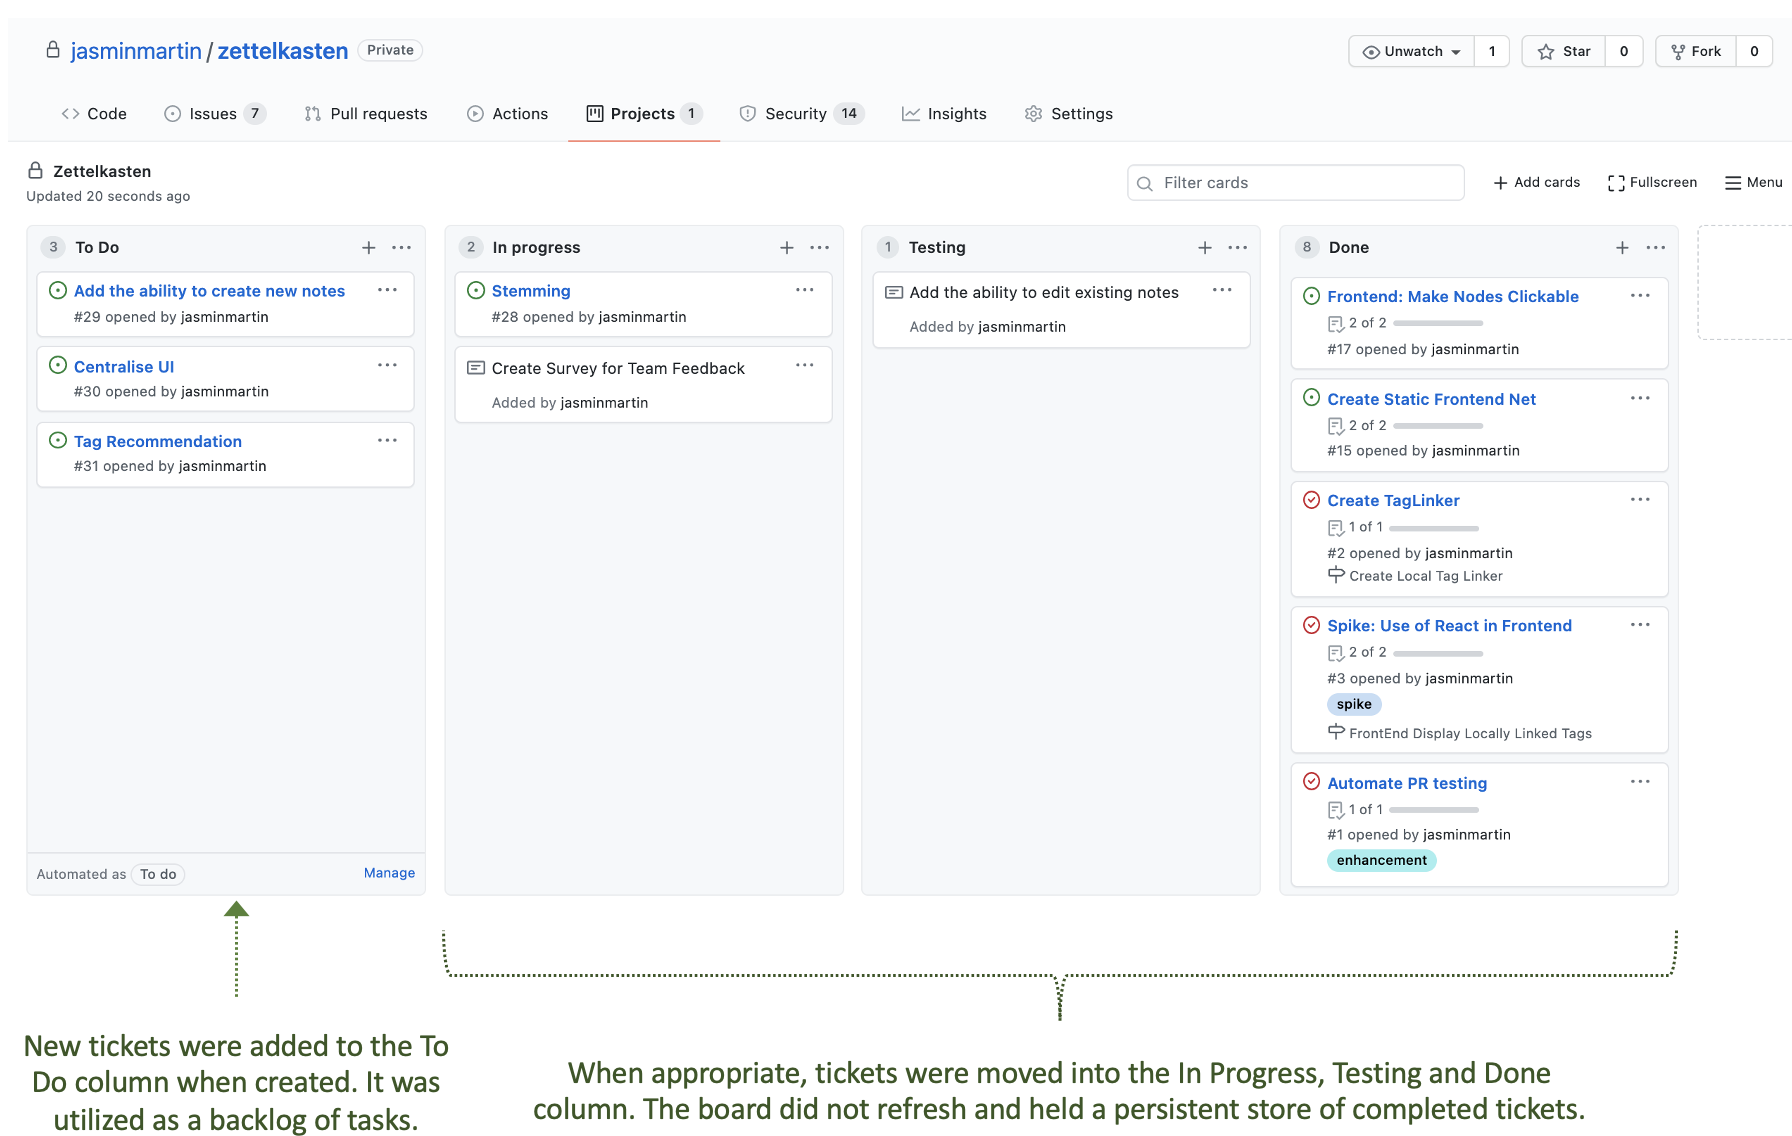
\includegraphics[width=1\textwidth]{images/methodology-ticket.png}
  \caption{The GitHub KanBan board used to track upcoming and completed tickets.}
\end{figure}

\begin{figure}[!htb]
  \centering
      \includegraphics[width=1\textwidth]{images/methodology-ticket-2.png}
  \caption{Each ticket outlined criteria which defined when a card could be completed.}
\end{figure}

\subsection{Incorporating User Feedback}

The incorporation of user feedback is a key tenant of agile development. Both oral and written feedback was captured during the development of Atlas. Once the minimal viable product was complete, the author showcased the application and collected initial feedback in a survey. The survey captured mainly quantitative data, as closed multiple choice questions prompted the respondent to rate the showcased user experience. Qualitative feedback was captured too, in a series of open questions which enabled the user to give more detailed opinions on the current and upcoming features. Both types of data were analysed to provide the author with an idea of the user’s needs and preferences. The results of the survey influenced the features incorporated into the second version of the application, and resulted in the refinement of the features included in the minimal viable product.

Further feedback was captured in the form of interviews and a focus group. As these two types of data collection required real-time feedback, they prompted more honest and detailed responses than the initial survey. This data also enabled the users to utilise Atlas themselves which in turn identified any difficulties with the user experience. Live data collection was particularly important for the development of Atlas as only a single developer created and designed the product, therefore other perspectives and viewpoints on the functionality made the product more valuable to a larger audience. The author decided to schedule a focus group for the end of version 2 development and later interviews for version 3 because interview can probe into more detailed answers. The notes on the opinions, questions, and ideas were analysed to determine any recurring themes which were addressed in the later versions of Atlas.

\newpage
\section{Requirements and Design}

Here the author describes the requirements solicitation process which shaped the design of Atlas. The initial product idea stemmed from the authors personal experience of struggling to comprehend a large, complex, hierarchical file system. As a result, the initial requirements were largely formed from the authors desire to demonstrate the benefits of generating the Atlas Web structure. Later iterations of Atlas incorporated user feedback - following the agile ethos of continuously tailoring the product to the user needs (Stellman and Greene, 2008). In this section, the author details how the user feedback influenced each iteration of the product.

\subsection{Iteration 1: MVP Concept}

The base functionality of Atlas was demonstrated in the minimal viable product (MVP). A MVP is a product with enough features to attract customers to validate the base functionality. The key purpose of a MVP is to enable the maximum amount of user feedback with the least amount of effort (Ries, 2009). The author’s personal experience of struggling to comprehend complex file systems formulated the base functionality of the MVP concept. The MVP was targeted towards adults with low technical experience. This demographic was selected as the research into competitor products revealed the popular knowledge management tools expected a moderate degree of technical literacy (see Strategic Rationale and Business Case section). As a result, the author designed a simple and accessible user interface and purposefully limited the number of steps in the user journey required to generate the Atlas Web (Figure 10). 

\begin{figure}[!htb]
  \centering
      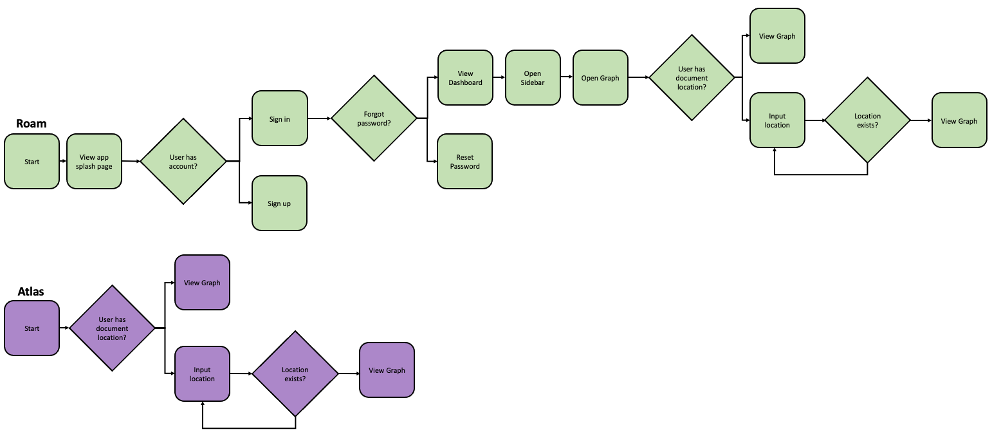
\includegraphics[width=1\textwidth]{images/userflow.png}
  \caption{To reduce the technical experience required to use Atlas the author simplified the user flow. Here the author compared the user journeys of graph generation for Atlas and it's competitor product Roam.}
\end{figure}

The author recognised the key features of Atlas with the aid of product wire frames (Figure 11). The original design of the Atlas web connected documents with common keywords; and displayed both the keyword and the name of the document on the Atlas web. The Atlas Web was designed to clearly depict the keywords in orange boxes, and documents in multi-coloured circles. From this visual depiction, the author recognised the two key functional requirements to be the ability to form relationships between documents and keywords (F1) and the ability to display the Atlas web on the user interface (F2) (Table 3). These feature were prioritised so the MVP could be quickly developed to demonstrate to users.

\begin{figure}[!htb]
  \centering
      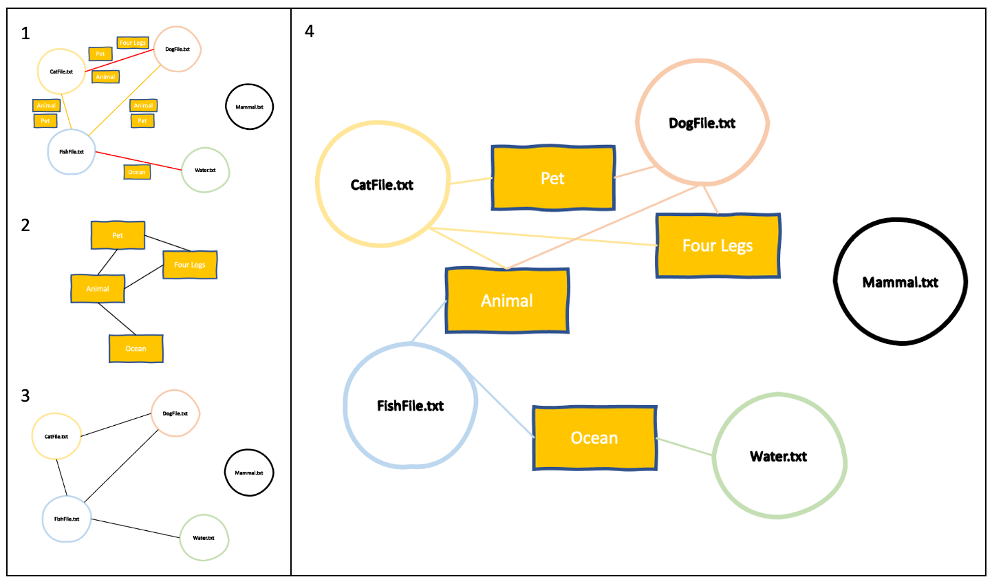
\includegraphics[width=1\textwidth]{images/wireframe.png}
  \caption{The development of initial wire frame of the Atlas web demonstrated the connections between documents with common keywords. The author experimented with different designs before settling on the circled document, boxed keyword arrangement (4).}
\end{figure}

Before developing Atlas, the author explored the requirements in greater detail with the aid of use cases and use case descriptions. Use case descriptions illustrate the behaviour of a system, without specifying how they are implemented (Hoda et al., 2008). On each iteration of the application, the author defined the use case descriptions for new functional requirements to help envision the technical implementation of the new features (Tables 3-6).

//table

Although the resulting product did not match the MVP wire frame exactly due to library limitations (Figure 12), the author successfully implemented the initial functional requirements.

\begin{figure}[!htb]
  \centering
      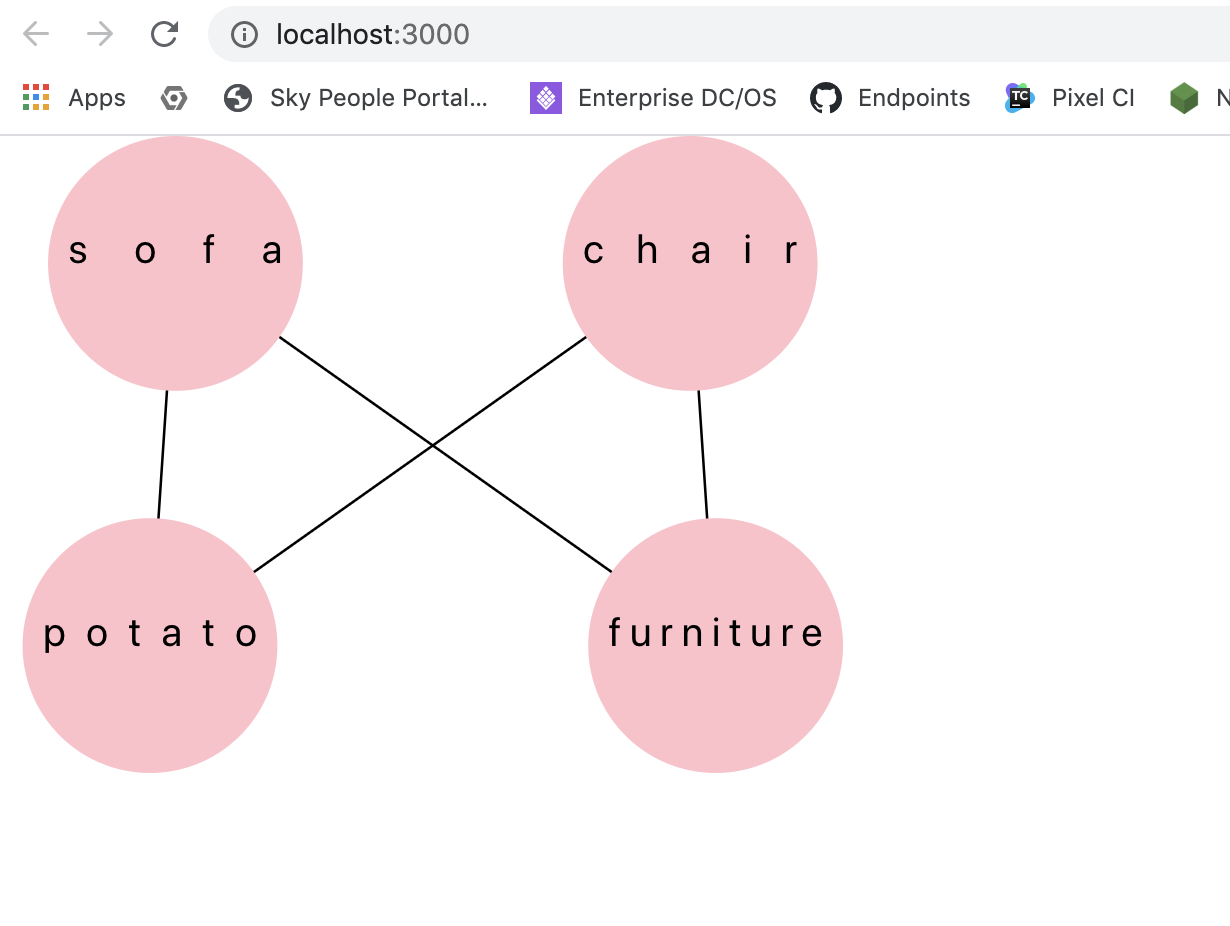
\includegraphics[width=1\textwidth]{images/mvp-frontend.png}
  \caption{The resulting MVP product could connect documents based on keywords.}
\end{figure}


\begin{table}[]
\centering
\caption{The functional requirements and use cases that defined the minimum viable product.}
\label{tab:my-table}
\resizebox{\textwidth}{!}{%
\begin{tabular}{|l|l|p{4.5cm}|p{3cm}|p{6cm}|}
\hline
\textbf{Phase} & \textbf{Id} & \textbf{Functional Requirement} & \textbf{Use Case} & \textbf{Use Case Description} \\ \hline
\textbf{MVP} & F1 & To   form relationships between tagged words & Calculate   keyword links & When   the system is provided with a directory, it must parse the file contents and   calculate the Atlas Web. \\ \hline
\textbf{MVP} & F2 & To   display relationships on the user interface & Display   Atlas web & A   user should be able to view the Atlas Web that displays all of the files and   the relationships between them. \\ \hline
\end{tabular}%
}
\end{table}

\subsection{Iteration 2: Showcase and Survey}

To formulate the requirements used to iterate upon the MVP, the author showcased Atlas to members of their department. The presentation described the project aims and included a demonstration of the MVP Atlas Web (Figure 13). The dual purpose of the presentation was to inform colleagues of the authors apprenticeship work, and to collect feedback on the MVP. The presentation was followed by a survey which would inform the author of the success of implemented requirements and influence the development and prioritisation of future requirements. Due to Covid-19 restrictions, the showcase was held on Microsoft Teams with an audience of 15 members of the author’s organisation. 

\begin{figure}[!htb]
  \centering
      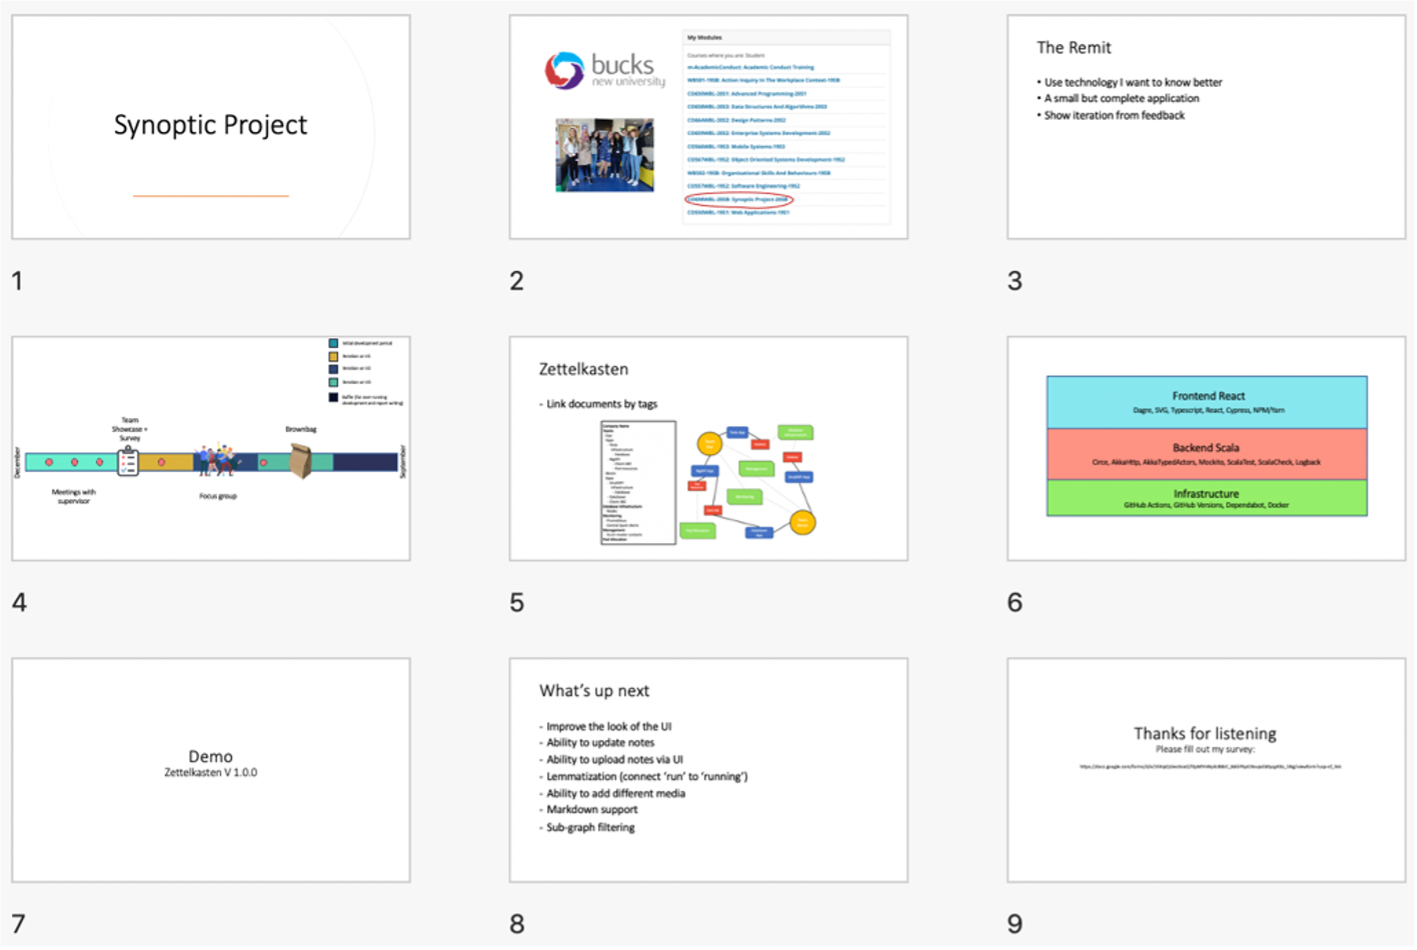
\includegraphics[width=1\textwidth]{images/showcase.png}
  \caption{The slideshow presentation showcased the project background and the MVP  to prospective users.}
\end{figure}

The author purposely chose to showcase the MVP to members of the department early in the development process to generate an awareness of the project to the department. The author hoped this could lead to opportunities to collaborate with members of the department and could help find a team to maintain the application on completion. A stratified sample of 25 members of the department were invited to the showcase, but unfortunately 10 members could not attend. The demographic of the audience was largely male (80\%) and consisted of employees in technical roles. The author was aware that this population may not be reflective of the final user base, and could show a bias toward both male and technical opinions. This limitation was reflective of their organisations population. However, the author noted if the product was to be utilised in technical organisations, this would likely be the demographic that utilised the product.

After the showcase, attendees were asked to complete a survey (Appendix 1). The survey offered a low cost and convenient mechanism for generating a large amount of data (Jones et al., 2013). It had two key purposes – the first was to understand whether the audience had understood the purpose of the current MVP concept, and the second was to give the opportunity to suggest future features. This data would influence the design and future functional requirements of Atlas. The survey contained primarily closed questions used to collect quantitative data on topics such as rating the existing product user interface, the user journey and the users desire to user the application. Open questions enabled the respondents to suggest new features that the author may not have previously considered. The data was compiled and analysed to influence the priority of the next functional requirements (Figure 14).

\begin{figure}[!htb]
  \centering
      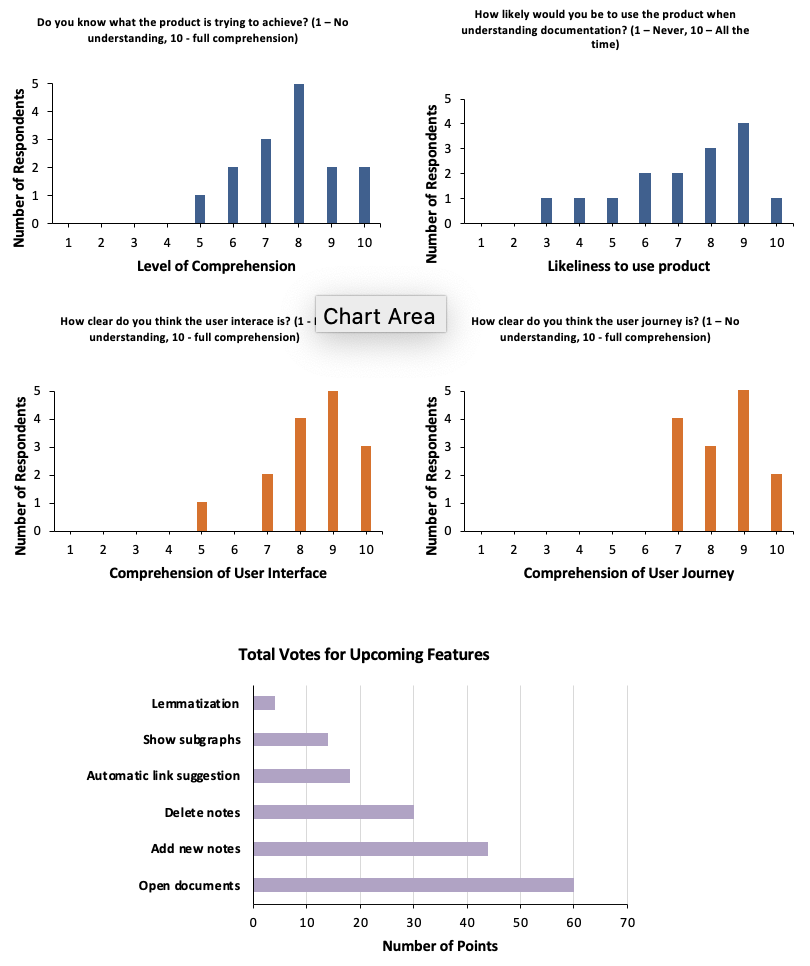
\includegraphics[width=1\textwidth]{images/survey-results.png}
  \caption{The minimal viable product survey revealed users comprehension of the current product and future features that they would like to see implemented.}
\end{figure}

The data analysis revealed that current MVP concept was well understood; as the average audience member rated product comprehension at a 7.9, user interface comprehension at  9.1 and user journey comprehension at 8.8. The audiences rated their likeliness to use the product as 7.1. Comments from the survey suggested this lower value may stem from concerns that the Atlas Web may not be able to handle larger document structures than demonstrated. The author ensured to demonstrate Atlas Webs with more data in the future. Comments on the current MVP design highlighted the fact that Atlas web was not centralised.

The survey prompted users to vote for Atlas’s upcoming features. By far, the most voted for new feature was the ability to open the documents within the application (F3). The second and third most voted features were the ability to add (F4) and delete notes (F5). These formed the three functional requirements to be implemented into the next iteration of Atlas (Table 3). Interestingly, three survey respondents suggested the same additional feature – the ability to zoom in on the Atlas web interface. This ability proved more popular than the author’s suggested sub-graph feature. Although this feature was not incorporated into the second iteration of Atlas due to workload, the author highlighted this as a potential feature in the upcoming focus group.

\begin{table}[]
\centering
\caption{The functional requirements and use cases that defined the second iteration of Atlas.}
\label{tab:my-table}
\resizebox{\textwidth}{!}{%
\begin{tabular}{|l|l|p{4.5cm}|p{3cm}|p{6cm}|}
\hline
\textbf{Phase} & \textbf{Id} & \textbf{Functional Requirement} & \textbf{Use Case} & \textbf{Use Case Description} \\ \hline
\textbf{It. 2} & F3 & To   view document content & View   document content & A   user should be able to click on an Atlas web document to open a modal which   will display the document contents. \\ \hline
\textbf{It. 2} & F4 & To   add a new document & Add   document & A   user should be able to add a new document to the Atlas Web. \\ \hline
\textbf{It. 2} & F5 & To   delete an existing document & Delete   document & A   user should be able to delete an existing documents from the Atlas Web. \\ \hline
\textbf{It. 2} & F6 & To   edit document content in the Atlas Web & Edit   document & A   user should be able to see the instruction guide when they first open the   application. \\ \hline
\end{tabular}%
}
\end{table}

To aid the development of the second iteration, the author introduced a basic user actor to the system (Figure 12). Atlas only catered to a single actor, as the primary purpose of the application was to automatically transform the file system into the Atlas web. As there was no concept of an admin user, all of the functionalities were carried out by the basic user.

\begin{figure}[!htb]
  \centering
      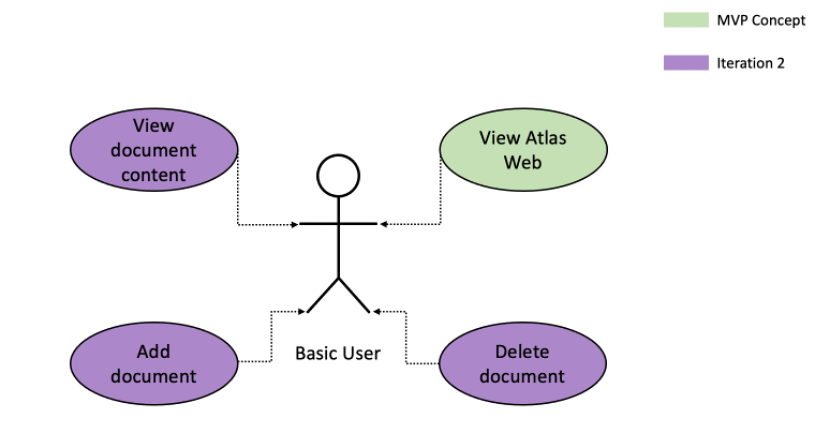
\includegraphics[width=1\textwidth]{images/actor-diagram.png}
  \caption{diagram showing the functionalities carried out by the basic user.}
\end{figure}

\subsection{Modal and Atlas Web Design}

Before the implementation of iteration 2 of Atlas, the author created wire frames of the document modal that would be used to display document content (F3). The wire frame provided a visual guide for the developer that ensured the element positions were both appealing and clear (Stone et al., 2005). The author also used the wire frames to update the design of the Atlas Web based on feedback from the survey.

Due to aforementioned library limitations, the Atlas Web represented both documents and keywords as circles. The author liked this design, as circles are universally known as clickable buttons, therefore they enticed  users to click on them. Relationship between the files were represented by lines. Lines were chosen over arrows, as not to overcrowd the screen or make the system appear overly complex (Najjar, 1998). The user is able to add a new document by pressing the New File button from the Atlas Web user interface (Figure 16A). 

When a user clicked a circular node, a modal appeared with the file contents (Figure 16B). The appearance of a modal was chosen, rather than a new page, as it provided a smoother transition. The user could easily click on the background Atlas Web or the closing ‘X’ to close the modal. Therefore the user should feel confident navigating the product. Furthermore, the modal was chosen as it provided a distinct experience from the traditional file system which opens different files in different application windows.

The author decided to keep the design of the application simple and enable the user to both edit and delete the document within the modal view (Figure 16C). To edit a document, the user clicked the body or title of the modal. This mobile-centric approach was taken as it reduced the number of buttons on the user interface. The save and delete buttons in edit mode allowed the user to update the document accordingly.

\begin{figure}[!htb]
  \centering
      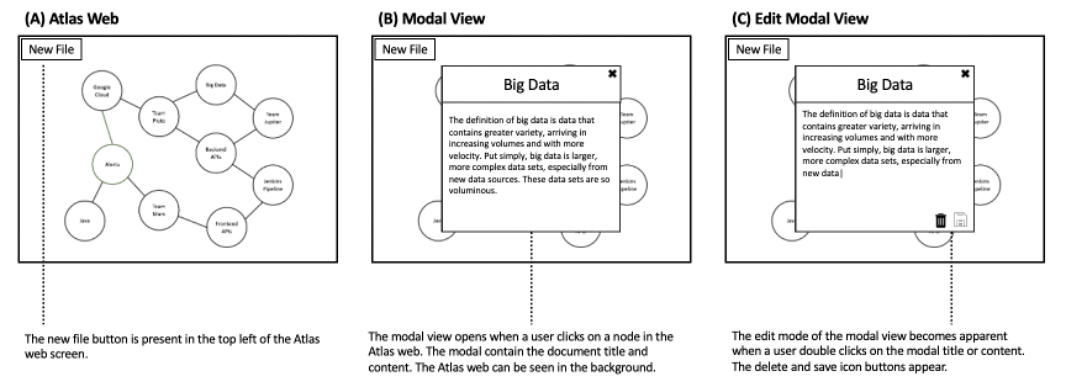
\includegraphics[width=1\textwidth]{images/modal.png}
  \caption{Wireframes representing the Atlas Web (A), the modal view (B), the edit modal view (C).}
\end{figure}

The author completed the development of the modal, and managed to produce a design similar to the intended wire frames (Figure 17).

\begin{figure}[!htb]
  \centering
      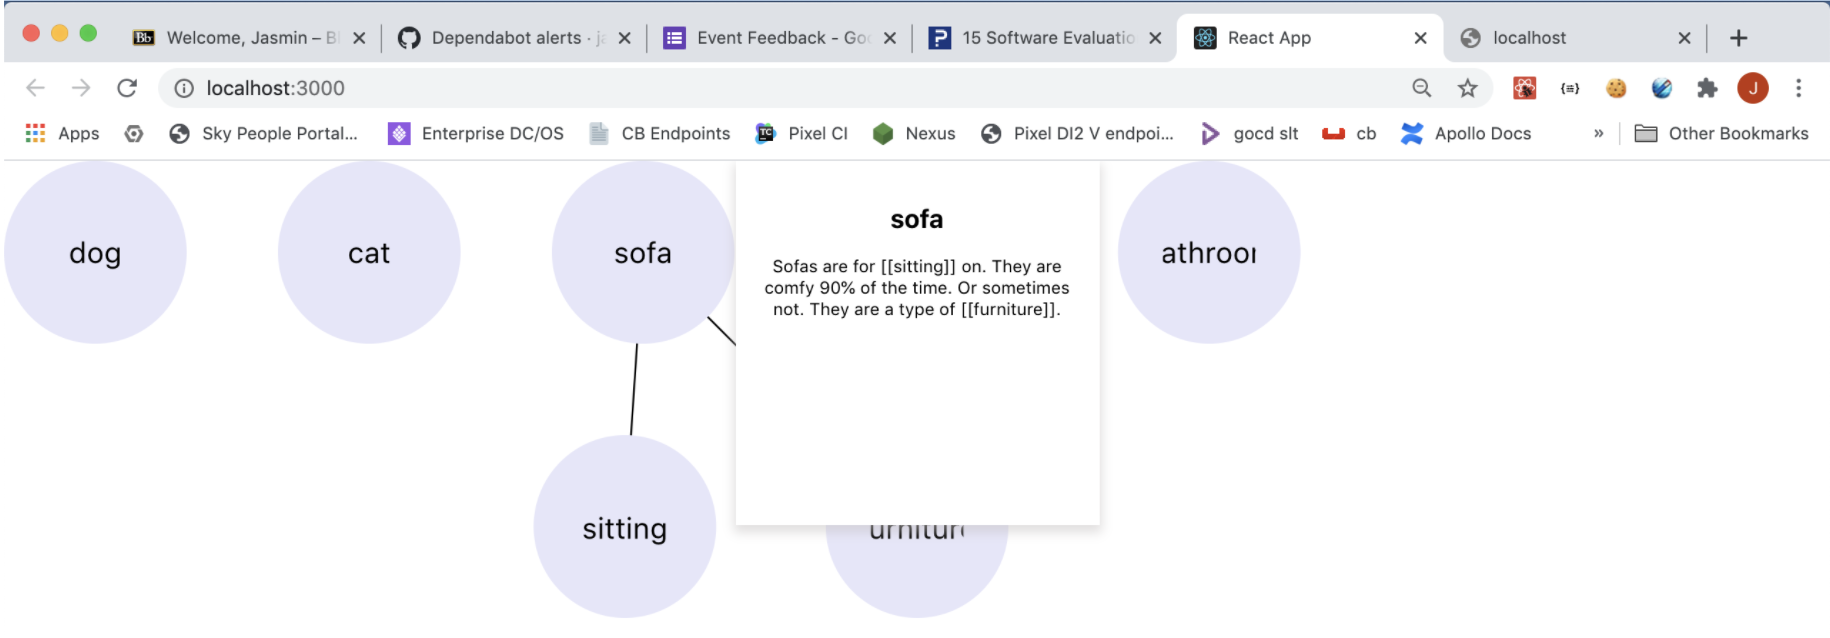
\includegraphics[width=1\textwidth]{images/modal-screenshot.png}
  \caption{The modal displaying the document content opened when a user clicked on a document node.}
\end{figure}

\subsection{Iteration 3: Focus Group}

Once the second iteration of the product had been developed, further requirements were gathered with the feedback from a focus group. The aim of the focus group was to gather several different feelings and perspective on the product (Gibbs, 1997). The focus group consisted of 6 members of the organisation, and included a small introduction to the product, followed by a demonstration that enabled users to interact with the product. Each user was encouraged to interact with the application so that they experienced all elements of the user journey. With permission from the users, the session was recorded. This enabled the author to engage with the users during the session and then replay the footage to make notes of any comments or concerns about the user experience (Appendix 1). To ensure the focus group was reflective of the user base, a stratified sample of users across the organisation was selected, to ensure a broader career range and gender ratio was selected. 

The output of the qualitative data was analysed to find common sticking points with the application. For instance, three members of the group initially struggled to understand how the application translated the traditional file system into the web. It was suggested an instruction guide could alleviate this issue (F7). Furthermore, the author included a larger data set in the demonstration and as a result, the focus group reported it was difficult to comprehend the whole Atlas web. The group responded positively to the suggestion of a zoom in feature to alleviate this issue (F8). The group also highly recommended the ability to automatically suggest new connections, as one member iterated that they would not find the product beneficial unless it had this additional ability (F9). The author prioritised these 3 new suggestions by their ease of implementation as they were aware of time constraints.


\begin{table}[]
\centering
\caption{The functional requirements and use cases that defined the third iteration of Atlas.}
\label{tab:my-table}
\resizebox{\textwidth}{!}{%
\begin{tabular}{|l|l|p{4.5cm}|p{3cm}|p{6cm}|}
\hline
\textbf{Phase} & \textbf{Id} & \textbf{Functional Requirement} & \textbf{Use Case} & \textbf{Use Case Description} \\ \hline
\textbf{It. 3} & F7 & To display an instruction guide & Display instructions & A user should be able to see the instruction guide when they first open the   application. \\ \hline
\textbf{It. 3} & F8 & To zoom into the Atlas Web & Zoom into Atlas web & A user should be able to zoom into different parts of the Atlas Web. \\ \hline
\textbf{It. 3} & F9 & To automatically suggest new connections & Suggest new notes & The system must be able to suggest potential connection based on common words. \\ \hline
\end{tabular}%
}
\end{table}

An unexpected development that stemmed from the focus group was the change in the products name. Originally, the product had been named ‘Zettelaksten’, after the author of the underlying transformation algorithm. The group reported the name had complex connotations and did not describe the product purpose well. For the fourth iteration of development, the author renamed the product to Atlas, as it was simpler and better aligned with the products purpose – the creation of knowledge maps.

The author successfully implemented the instruction guide (Figure X) and the zoom functionality (Figure X) and presented these features in the next iteration of development.

\subsection{Iteration 4: Interviews}

The author had planned to conduct interviews with several members of the organisation to form future requirements and gather feedback on the third iteration. Interviews are particularly advantageous as the author is able to adapt their line of query to the interviewees responses (Gibbs, 1997). Unfortunately, the author only had time to interview one colleague, due to time restrictions. The feedback from the interview was largely positive. The interviewee suggested one additional feature - the ability to group documents with similar names such as 'database' and 'databases'. This process is known as lemmatisation.

\begin{table}[]
\centering
\caption{The functional requirements and use cases that defined the fourth iteration of Atlas.}
\label{tab:my-table}
\resizebox{\textwidth}{!}{%
\begin{tabular}{|l|l|p{9cm}|p{3cm}|p{12cm}|}
\hline
\textbf{Phase} & \textbf{Id} & \textbf{Functional Requirement} & \textbf{Use Case} & \textbf{Use Case Description} \\ \hline
\textbf{It.   4} & F10 & To   stem similar words & Stem   document titles & The   system must stem similar keywords \\ \hline
\end{tabular}%
}
\end{table}

In order to implement the lemmatisation requirement (F11), the author used a sequence diagram to plan how to implement the stemmer (Figure X). Sequence diagrams demonstrate the interaction between systems over time (Fowler, 2003). This enabled the author to understand that when a user provided the location of a file system, the system could then identify the nodes and edges of the documents by parsing each file individually. The nodes would be stemmed when they were identified by the system.

\begin{figure}[!htb]
  \centering
      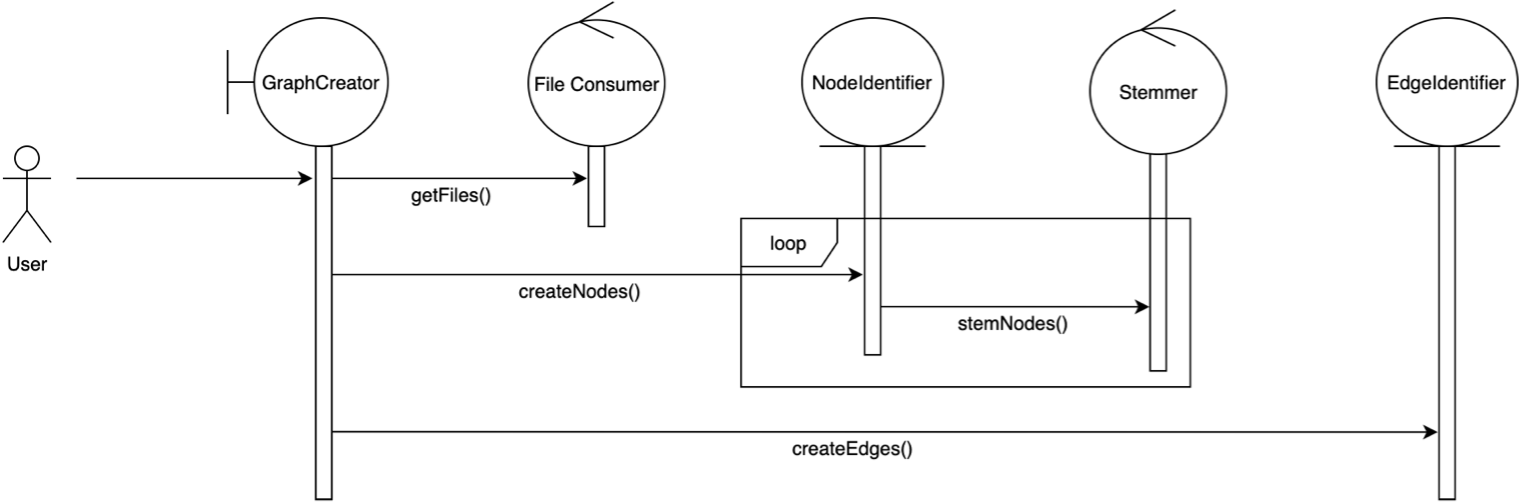
\includegraphics[width=1\textwidth]{images/sequence-diagram.png}
  \caption{The sequence diagram demonstrate how a user interacts with the system to create an Atlas web.}
\end{figure}

\subsection{Class Diagram with Entity Relationships}

To translate the use case descriptions into a technical design, the author consolidated class diagrams with the entity relationships schemas to demonstrate the relationship between the classes and objects within the system (Figure X). The author first created this diagram before the MVP concept was implemented, and extended it with future iterations of the application. The diagram was then used to guide the development of Atlas.

The case class diagram shows two key packages – the file consumer package consisted of the FileConsumer trait and LocalFileConsumer class, and the GraphGenerator package which consisted of eight objects and classes connected to the GraphCreator class. The GraphCreator class utilised the EdgeIdentifier and NodeIdentifier objects to produce the list of files and related nodes which in turn, generated the Graph displayed to the user. These objects were supported by the FilesAndTags class, with the resulting objects being combined by the GraphCreator. The NodeIdentifier object was further supported by the Stemmer object, which enabled the lemmatisation functionality.

\begin{figure}[!htb]
  \centering
      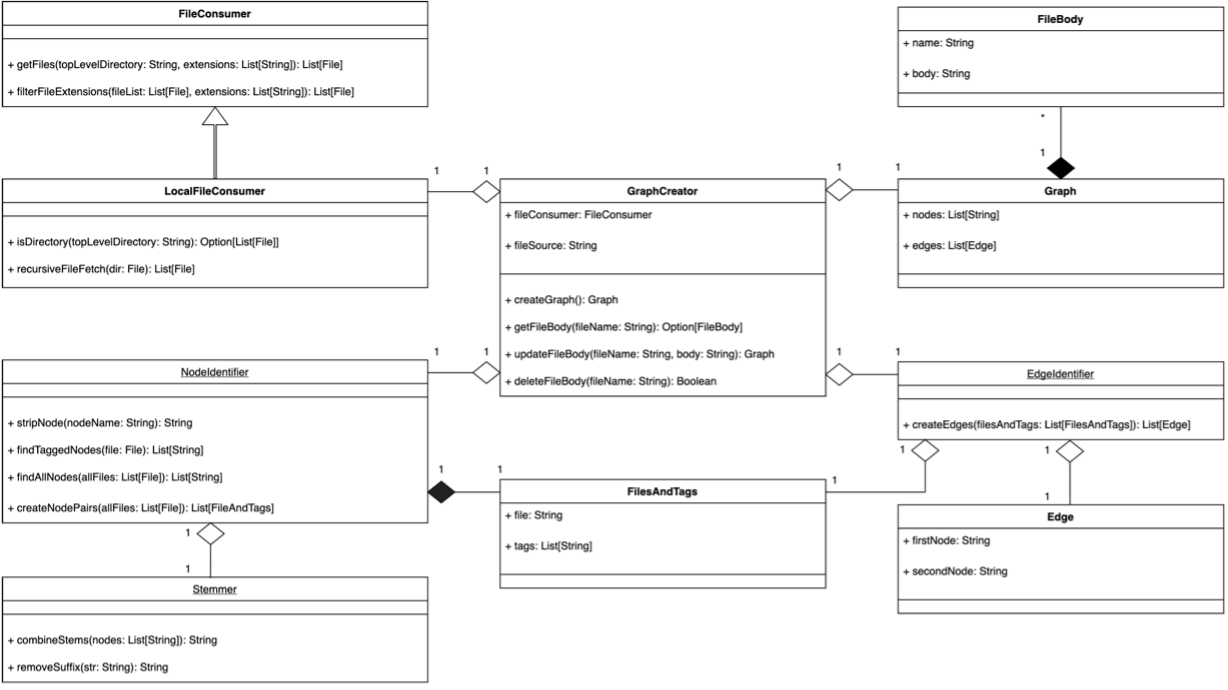
\includegraphics[width=1\textwidth]{images/entity-relationship.png}
  \caption{A combined case class and entity relationship diagram for the Atlas system.}
\end{figure}

\subsection{Non-Functional Requirements}

Whilst the functional requirements defined the behaviour of the application, the non-functional requirements described the system level attributes such as performance, security, usability and reliability (Augustine et al., 2005). Non-functional requirements are important as they can determine whether the user has a positive user experience. The non-functional requirements of Atlas were solicited throughout the development process (Table 6). The focus group elicited the importance of the user’s ability to understand and comprehend the applications features (NF1). The second and third non-functional requirements concerned with the security (NF2) and speed (NF3) of the application stemmed from the guidelines of similar applications (Addison-Wesley, 2003). The final non-functional requirement focused upon the developer experience (NF4). It was important to maintain a clean code base, as the application may have to be maintained by other members of the department. 

\begin{table}[]
\small
\caption{The non-functional requirements of Atlas.}
\centering
\label{tab:my-table}
\resizebox{\textwidth}{!}{%
\begin{tabular}{|l|p{6cm}|p{5cm}|}
\hline
\textbf{Id.} & \textbf{Non-Functional   Requirement} & \textbf{Example} \\ \hline
\textbf{NF1} & A user must be able to understand the Atlas   Web and be able to navigate the user interface with ease. & A user should be able to understand the   instruction of the application by reading the instructions. \\ \hline
\textbf{NF2} & The security of a system must keep the   customer information confidential and prevent any unwanted outside   interaction with the system. & User data must only be stored locally. \\ \hline
\textbf{NF3} & The application performance must respond   within a 500ms transaction time. & A user should be able to see a newly added node appear on the user   interface within 500ms. \\ \hline
\textbf{NF4} & The   application codebase must be well maintained and accessible for future   developers. & A linter will be used to reduce the amount of   errors and stylistic differences. \\ \hline
\end{tabular}%
}
\end{table}

\newpage
\section{Development}
\subsection{Time Management}

A total of four iterations of Atlas were developed. The first iteration, the MVP, was completed as planned in early January after 14 weeks of development. The three later iterations of the application did not meet the initial schedule, as they overran by 3-5 weeks each (Figure 16). Time management was highlighted as a low risk in the initial plan (R4), and as a result the author had added a 20\% buffer to all time estimates. Although all four iterations of the product were completed, the author had significantly less time finish the development and to complete the project report.

\begin{figure}[!htb]
  \centering
      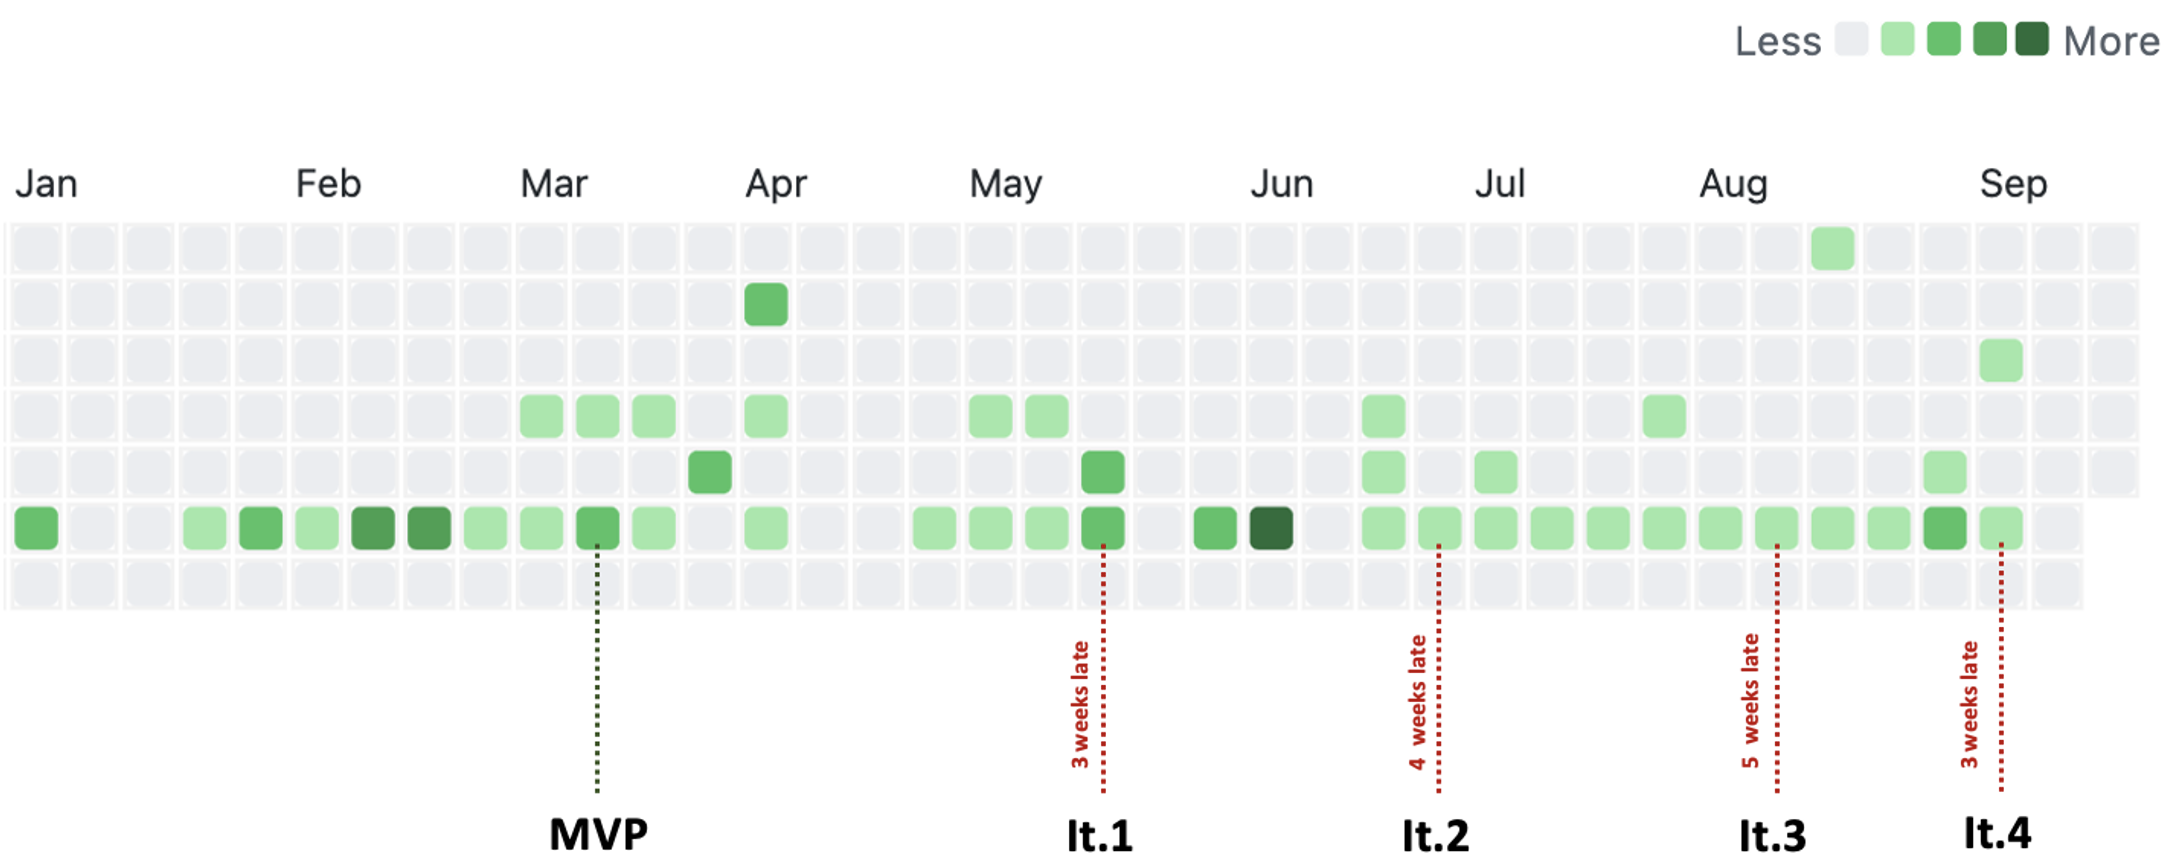
\includegraphics[width=1\textwidth]{images/timeline.png}
  \caption{Annotated GitHub commit chart demonstrates the successful completion of the MVP on schedule, followed by time slippage on the later iterations of Atlas.}
\end{figure}

The author had allocated half a day each week to the project to allow time for work on parallel university modules. This assumption proved inaccurate, as the high time demands of the parallel modules resulted in little time for project development. Unfortunately, due to high work demands outside of the apprenticeship, the product could not be developed as part of the authors daily work. As a result, the author found themselves developing the project outside of the allocated hours, which in turn made it difficult to gain momentum on each iteration. The additional task of writing the report led to later stages of development becoming particularly rushed. Fortunately, the Scrumban agile methodology enabled the author to prioritise important tasks and omit those not required to create a functionally complete product.

\subsection{Completed Functionality}

The author implemented 9 of the 10 functional requirements outlined in the original requirements and design section (Table 7). The automatic tag suggestion requirement (F8) was omitted due to the aforementioned time constraints. The author prioritised later requirements as the development of the automatic tag suggestion (F8) took significantly longer than expected. The author struggled to develop a solution which could efficiently store and identify words common to multiple documents. If this requirement was further developed, the author would research Scala frameworks which could store and manipulate large quantities of data such as the Play Framework (PlayFramework, 2021).

\begin{table}[]
\centering
\tiny
\caption{Functional requirements developed as part of Atlas.}
\label{tab:my-table}
\resizebox{\textwidth}{!}{%
\begin{tabular}{|l|p{8cm}|l|}
\hline
\textbf{Id} & \textbf{Functional Requirement} & \multicolumn{1}{l|}{\textbf{Completed?}} \\ \hline
\textbf{F1} & To   form relationships between tagged words & \cellcolor[HTML]{92D050}\checkmark️ \\ \hline
\textbf{F2} & To   display relationships on the user interface & \cellcolor[HTML]{92D050}\checkmark️ \\ \hline
\textbf{F3} & To   view document content & \cellcolor[HTML]{92D050}\checkmark️ \\ \hline
\textbf{F4} & To   add a new document & \cellcolor[HTML]{92D050}\checkmark️ \\ \hline
\textbf{F5} & To   delete an existing document & \cellcolor[HTML]{92D050}\checkmark️ \\ \hline
\textbf{F6} & To   display an instruction guide & \cellcolor[HTML]{92D050}\checkmark️ \\ \hline
\textbf{F7} & To   zoom into the Atlas Web & \cellcolor[HTML]{92D050}\checkmark️ \\ \hline
\textbf{F8} & To   automatically suggest new connections & \cellcolor[HTML]{EA5563}\\ \hline
\textbf{F9} & To   edit document content in the Atlas Web & \cellcolor[HTML]{92D050}\checkmark \\ \hline
\textbf{F10} & To   stem similar words & \cellcolor[HTML]{92D050}\checkmark \\ \hline
\end{tabular}%
}
\end{table}

\subsection{Completed Objectives}

The author implemented 3 of the 4 objectives that they initially set (Table 8). The author was satisfied that they had created a well-design product that efficiently aids users with the transformation of a file system into an Atlas Web (O2). Furthermore, they believe that with the implementation of user feedback, they developed a product that clearly depicts the relationships between documents (O3 and O1). Although the code for Atlas is open source on GitHub, the author did not deploy Atlas into a production environment due to time constraints (O4).

\begin{table}[]
\centering
\small
\caption{Objectives completed in the development of Atlas.}
\label{tab:my-table}
\resizebox{\textwidth}{!}{%
\begin{tabular}{|l|l|l|}
\hline
\textbf{Id} & \textbf{Objective} & \textbf{Completed?} \\ \hline
\textbf{O1} & Design a user interface that clearly depicts the   relationships between documentation. & \cellcolor[HTML]{92D050}\checkmark \\ \hline
\textbf{O2} & Develop a minimal viable product that can   transform a specified filesystem into the web interface. & \cellcolor[HTML]{92D050}\checkmark️ \\ \hline
\textbf{O3} & Gather and incorporate user feedback on the   minimal viable product and develop future iterations of the application. & \cellcolor[HTML]{92D050}\checkmark️ \\ \hline
\textbf{O4} & Release the product and make the code open source. & \cellcolor[HTML]{FFC000} \\ \hline
\end{tabular}%
}
\end{table}

\subsection{Spike: Front-end React Development}

During the development of the MVP, the author dedicated a day of development to a spike on front-end libraries. A spike is a method for evaluating the impact of new technology that enables the developer to become more confident with the desired approach (Agile Learning Labs, 2021). The author had highlighted their lack of experience with front-end development as a risk from the outset (R1), and as a result they wanted to explore different solutions for the generation of the Atlas web. This exploration would also help the author minimise another identified risk, the inability of the chosen technology to efficiently generate the Atlas web (R2).

The author explored two key solutions for front-end web generation. The first, was to create the Atlas web with their own React components. From utilising online resources, the author learnt that it was easy to create basic shape components in React such as the lines and circles which form the basis for the web. Creating the shapes without the aid of a library would lead to a light weight solution to web generation. However, shape manipulation in space proved difficult as the relative coordinates changed with the screen size and scale (Figure 17A). The second solution the author explored was the use of the Dagre library (Pettitt et al., 2013). Dagre is a JavaScript library that creates client-side graphs. The author configured the graph to form the Atlas Web (Figure 17B). Although using Dagre could limit the product extensibility, the author decided to implement it into the product as it provided a quicker and more efficient solution to generating the Atlas Web. Furthermore, choosing Dagre mitigated the risk of building a bloated codebase (R5).

\begin{figure}[!htb]
  \centering
      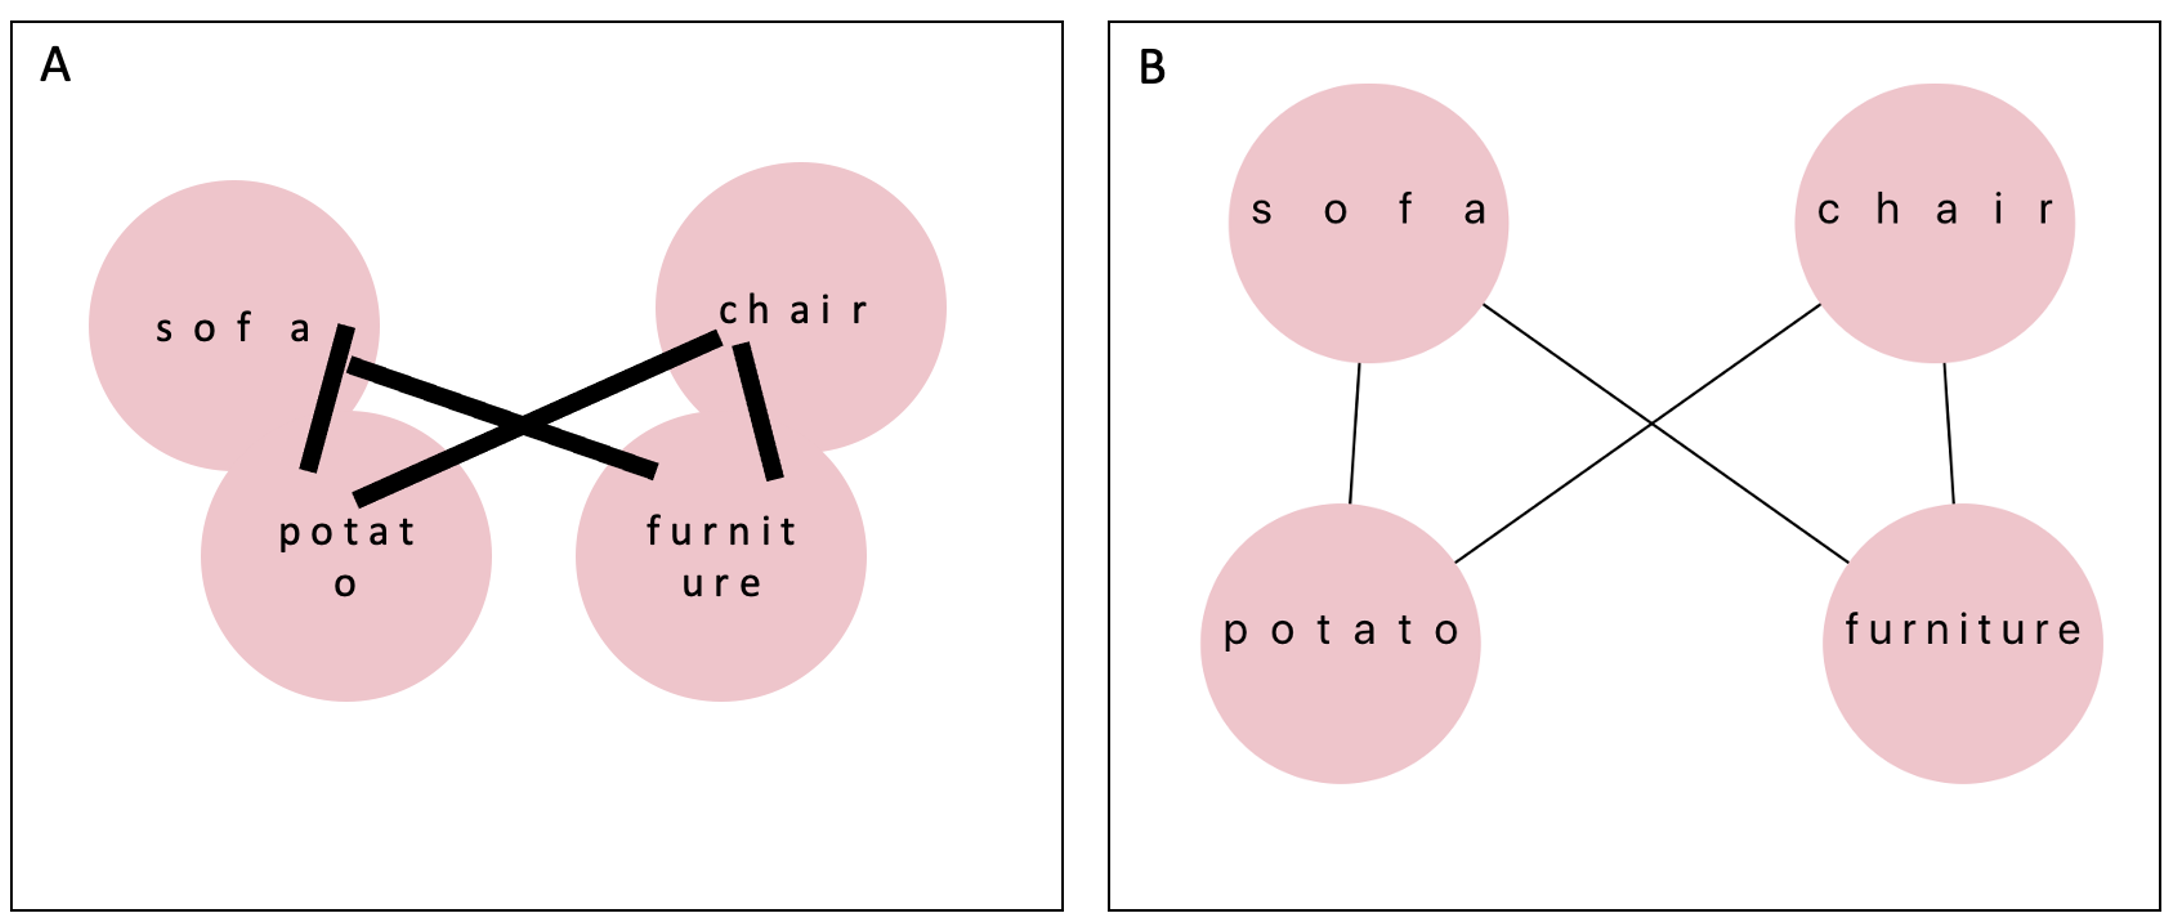
\includegraphics[width=1\textwidth]{images/dagre.png}
  \caption{The result of the front-end spike encouraged the author to use the front-end Dagre library (B) rather than create their own framework (A).}
\end{figure}

\subsection{Technical Issue: Requirement of a CORS Handler}

As part of the development of the MVP concept, the author was confronted a communication issue between the front-end and the back-end of Atlas. Atlas was designed to be segregated to simplify the development between the two different areas and to enable each to be scaled individually. However, the communication between the two was initially blocked by the presence of a Cross-Origin Resource Sharing (CORS) Policy error. CORS is a security mechanism in modern browsers that controls the access of resources from outside of the domain (Mozilla, 2021). When the author created the front-end server to invoke the back-end CRUD requests, they did not realise that CORS would invoke an OPTIONS security request before sending the intended CRUD call. As the back-end was not configured to handle the OPTIONS request, it resulted in a CORS error (Figure X).

\begin{figure}[!htb]
  \centering
      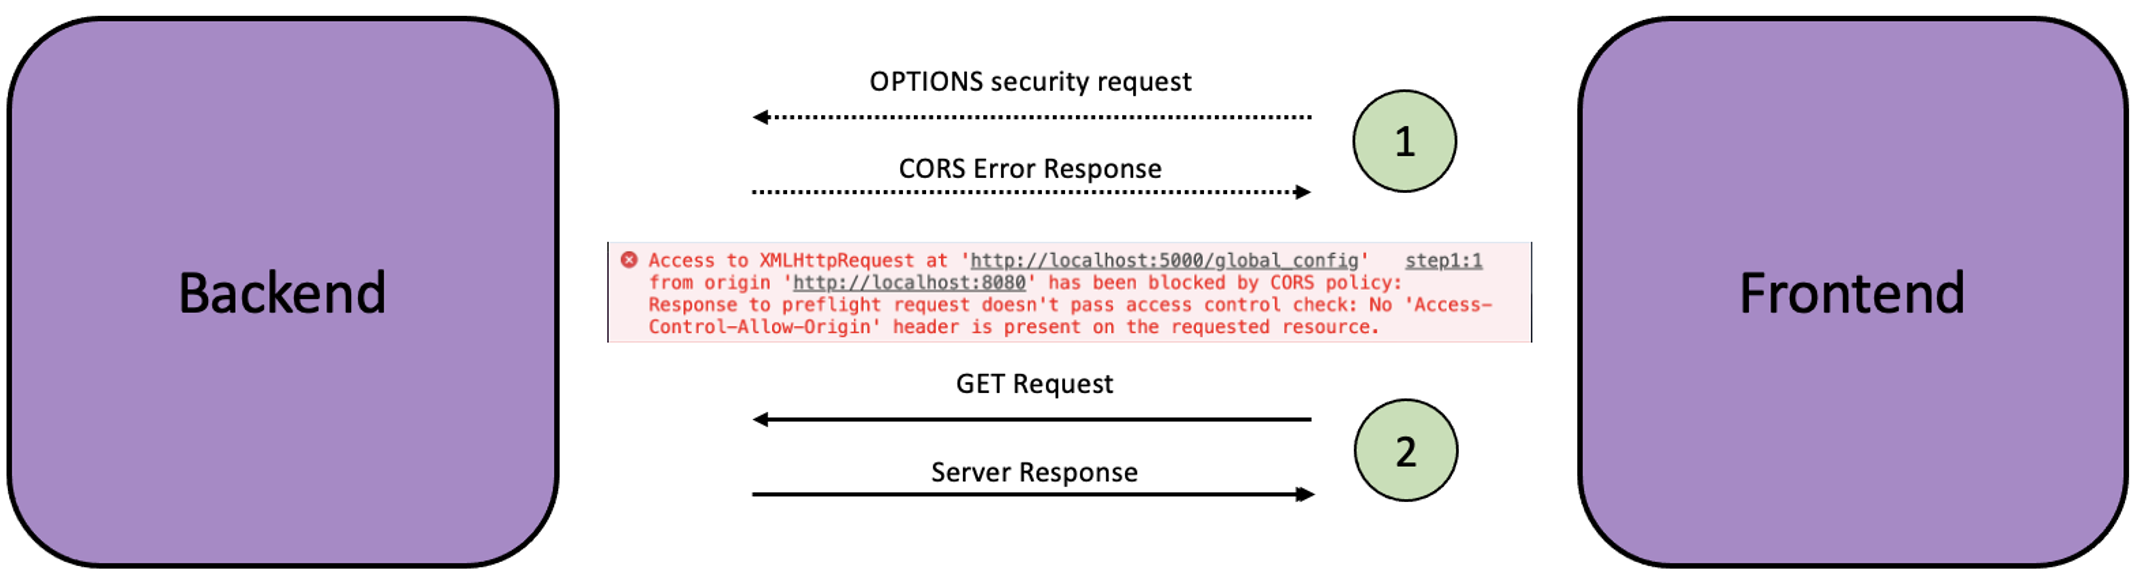
\includegraphics[width=1\textwidth]{images/cors.png}
  \caption{The author faced the technical issue of a CORS error as the backend was not configure to handle OPTION requests.}
\end{figure}

To solve the CORS policy error, the author implemented a CORS Handler trait to wrap the back-end server. This class enabled OPTION requests to the back-end and added the correct response headers to validate the security request. The author had not anticipated the risk of front-end-back-end connection issues as they previously had only interacted with front-end systems using cURL requests. Therefore, this error provided the author with the opportunity to learn about browser security mechanisms. 

\subsection{Technical Issue: Generating Test Data}

In order to test the ability for the back-end to generate the Atlas Web from a file system, the author created a series of unit tests which parsed a local file system. As more tests were added to the project, the test results became inconsistent. This was because certain tests invoked PUT requests to update the document contents, which caused subsequent tests to form incorrect assertions about the document contents. To make the tests stateless, the author created a utility class which could create a test file system. The utility class was invoked before each unit test was ran. The re-creation of the file system ensured that each test had a consistent environment which had not been manipulated by previous tests. Furthermore, it enabled the author to omit the test file system from the repository which reduced the test folders complexity. Therefore, the author learnt the importance of creating clean, stateless unit tests.

\subsection{Methodology Issue: Balancing Scrumban Roles}

Overall, the Scrumban methodology complemented the development of Atlas, as it enabled a flexible workflow that responded to the addition of new requirements. However, the author found it challenging to perform all of the roles required to maintain the Scrumban framework. As the author played the role of both the developer and the product owner, they were required to maintain the responsibilities of both roles. Therefore, in addition to maintaining the Scrumban board, creating the backlog and handling the workflow, they had to also develop, test and deploy the software. Therefore, during busier periods, the Scrumban board was not updated to reflect current work as the author prioritised development over management practices. In an attempt to maintain the Scrumban methodology, the author organised their apprenticeship work so that before the work period began, the author updated the Scrumban board.

\newpage
\section{Testing and Security}
\subsection{Testing Driven Development}

For the development of Atlas the author used test driven development (TDD). TDD is a software development practice that requires failing unit test to be created before the feature code is implemented (Figure X). Unit tests ensure that individual methods within the code display the intended behaviour. In TDD, software requirements are first converted into test cases before the author codes the solution to the new functionality. This structure forces the developer to think about the intended behavior of the feature and the design of the application. In turn, this results in simpler and more efficient code as the developer prioritises the design of the external interfaces (Fowler, 2003). Furthermore, TDD can improve both the reliability and developers understanding of the code as the framework encourages purposeful and consistent test cases (Beck, 2003). Future developers whom work on the project can then use these test cases as a starting point for understanding the intended behaviour of the application.

\begin{figure}[!htb]
  \centering
      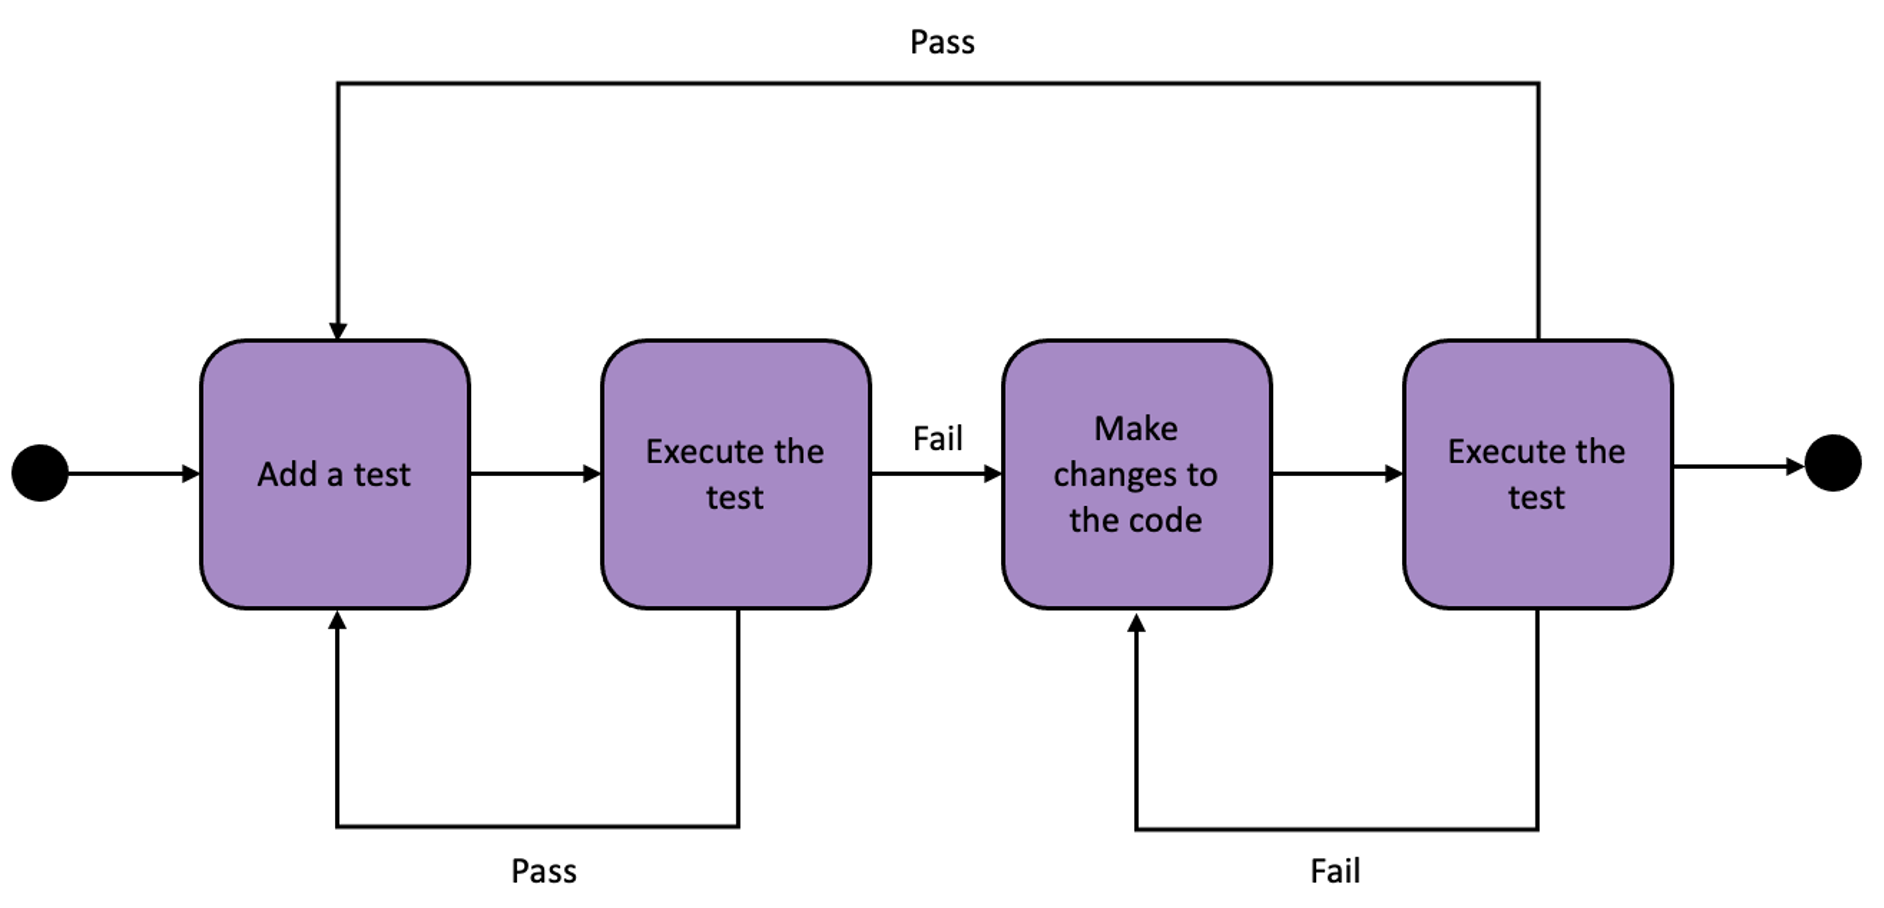
\includegraphics[width=1\textwidth]{images/tdd.png}
  \caption{The Test Driven Development cycle used in the development of Atlas enforced failing tests to be written before the code was implemented.}
\end{figure}

\subsection{Functional Tests}

In addition to unit tests, functional tests were implemented with every new feature. Functional tests validate the system works as intended by exercising the application as a whole (Juristo and Vegas,  2003). Thus, the functional tests closely mimicked the user journey and tested the system behaviour at a high level. In order to run the functional tests, the application was containerized with docker. Docker is software that packages an application and its dependencies into a virtual container (Docker, 2021). Docker can be ran on any operating system, as the virtual container ensures that tests were tun consistently in an isolated environment. As a result, this reduced the chance of technology-specific bugs. 

\subsection{Continuous Integration Pipeline}

It is important to regularly test applications during the development period to ensure no new bugs are introduced. The author introduced a continuous integration pipeline that automatically ran all unit and functional tests before a new feature was included in the application. The author created the pipeline as a GitHub WorkFlow. The WorkFlow ran all tests before a pull request could be merged into the master branch (Figure 20). The pipeline improved the code quality and reduced the number of manual steps required to release a new feature.

\begin{figure}[!htb]
  \centering
      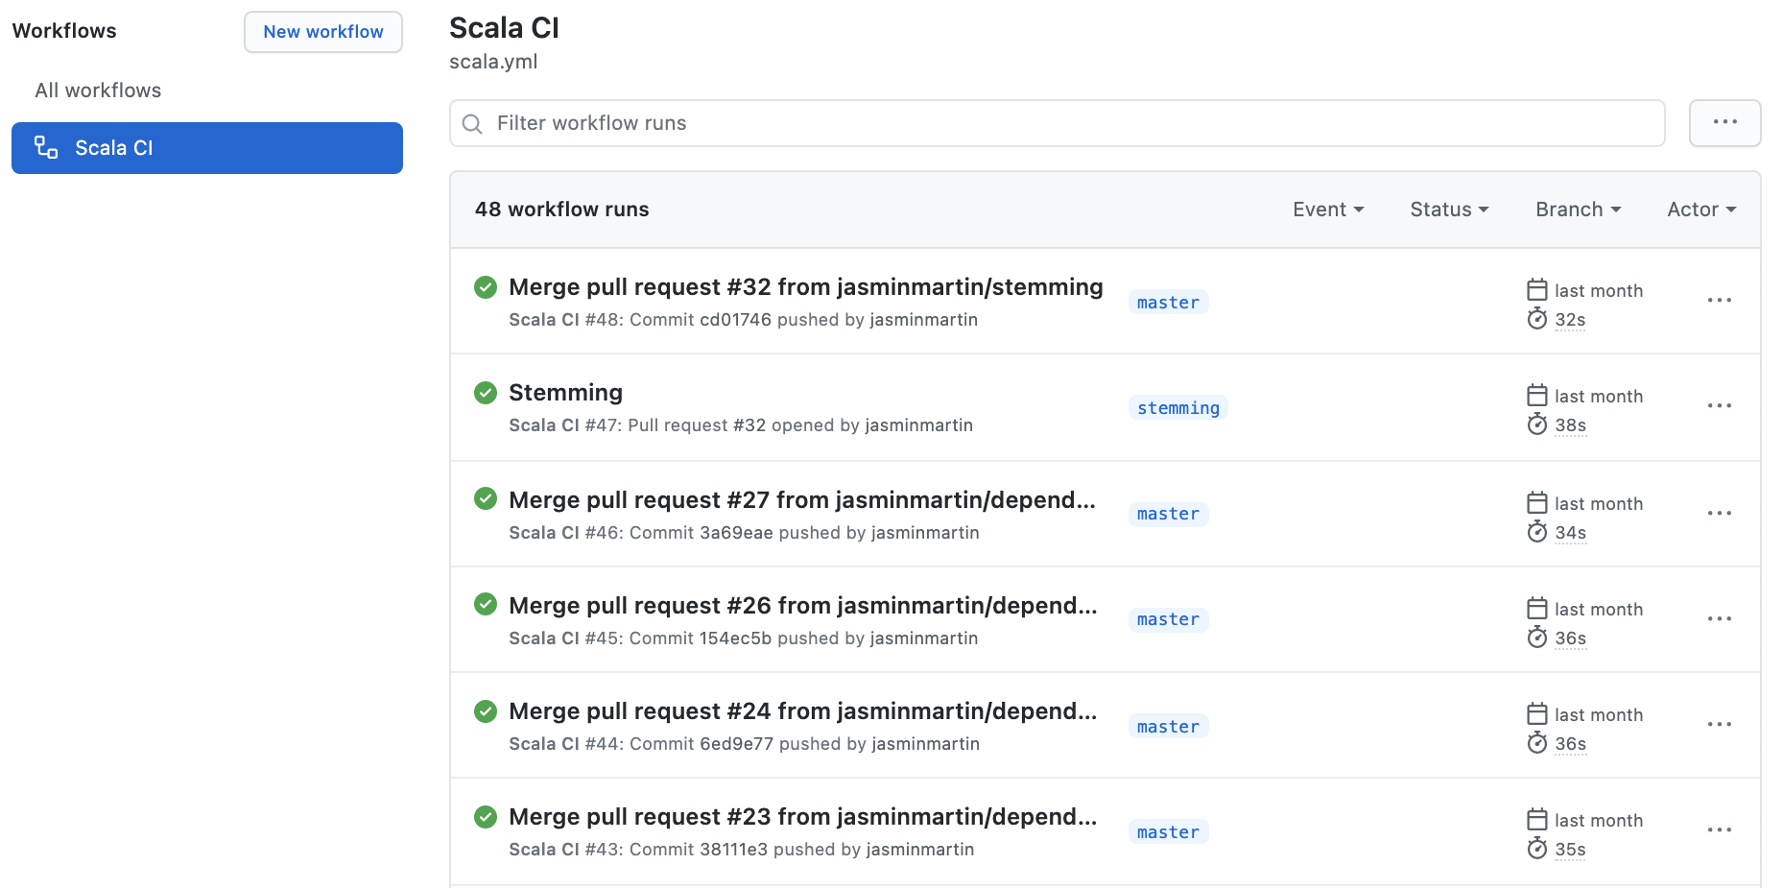
\includegraphics[width=1\textwidth]{images/scala-ci.png}
  \caption{The continuous integration pipeline for Atlas was created on a GitHub Workflow.}
\end{figure}

\subsection{Non-Functional Testing}
In addition to testing the functionality of the application, the author also tested its performance (NF3). It is important that the application could quickly respond to user commands to provide a smooth user experience. The author created a load test to simulate a user that adding and removing 500 documents to and from the Atlas Web within a period of 15 seconds. The author used Gatling to create the load test. Gatling is an open-source load-testing tool that measures the performance of an application (Gatling, 2021). The resultant report revealed that Atlas was able to handle the load without throwing any error or resulting in high latency's.

\subsection{Docker Image Vulnerabilities}

To improve the security of Atlas, the author scanned the application docker image for vulnerabilities. The author used Docker Scan to discover that the application initially contained 38 vulnerabilities; 8 of which were rated highly severe. The vulnerabilities stemmed from Atlas’s dependencies and transitive dependencies. These vulnerabilities could compromise the applications functionality or security. 

The Docker scan revealed a highly severe vulnerability in the openjdk-11 dependency. This dependency contained a bug that enabled unauthenticated attacker with network access via multiple protocols to compromise the Java SE (National Vulnerability Database – CVE -2021-2388, 2021). Another moderate rated vulnerability in the GNU C dependency enabled context-dependent attackers to cause a denial of service by exploiting regular expression bounded repetitions that bypass the intended limits (National Vulnerability Database – CVE -2010-4051, 2021). The vulnerable packages were upgraded to the safer versions to remove any dependency related security vulnerabilities (Figure X).

\begin{figure}[!htb]
  \centering
      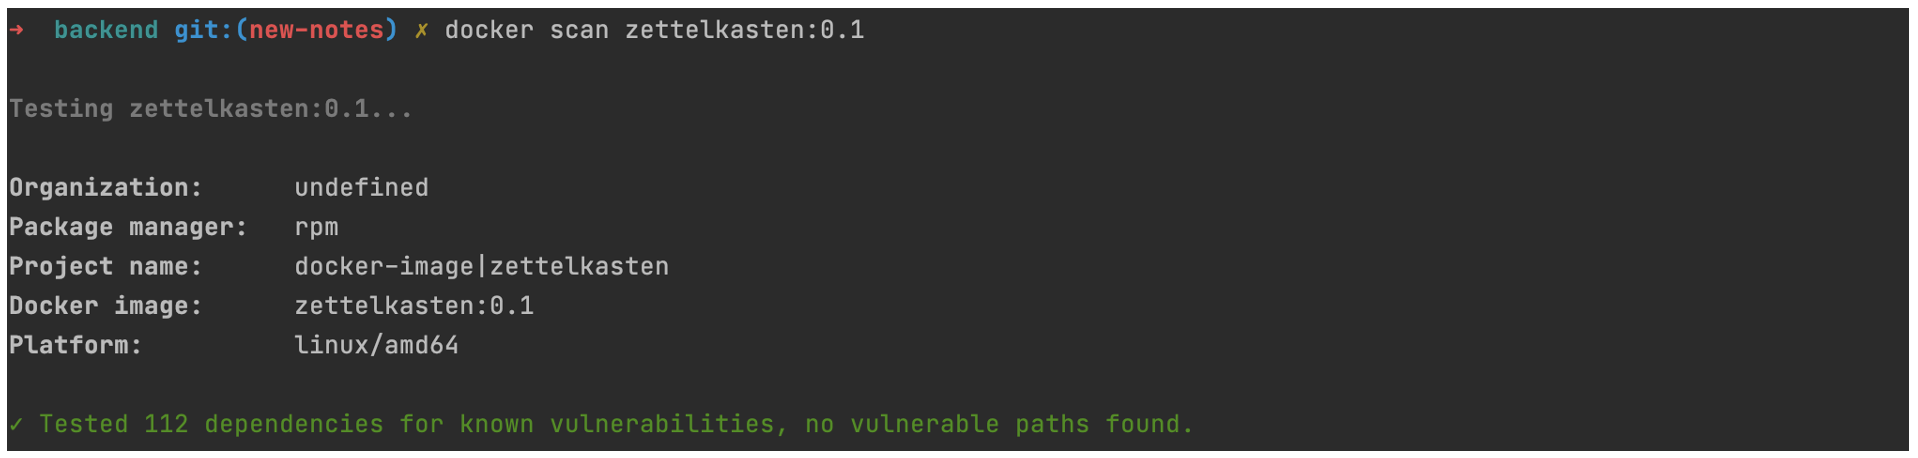
\includegraphics[width=1\textwidth]{images/vulnerabilities.png}
  \caption{A docker scan demonstrating no vulnerabilities found in the dependencies or transitive dependencies of Atlas.}
\end{figure}

In addition to upgrading the vulnerable dependencies, the author also changed the docker images base image to be distroless. Distroless images only contain the application code and the run-time dependencies. They lack the package manager, shells and operating system typical in a Linux distribution. Using a ditroless image not only reduces the number of potential packages containing vulnerabilities, but also makes the application less prone to surface attack as there is no shell to access the container (Moore, 2017). By removing the shell, a potential attacker cannot read any secrets on the container or secure information persisted such as user files (Figure X). It also prevents the installation of any untoward packages. The distroless image also has the additional benefit of being 35\% smaller than it’s non-distroless counterpart.

\begin{figure}[!htb]
  \centering
      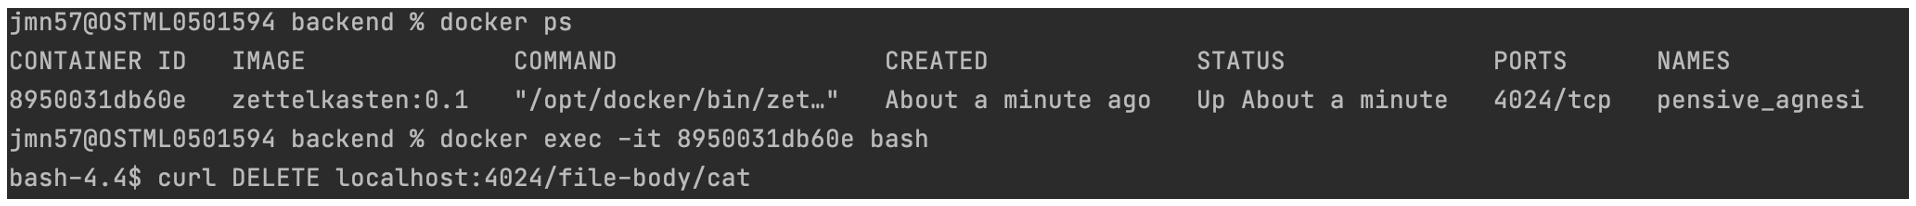
\includegraphics[width=1\textwidth]{images/distroless.png}
  \caption{An attacker could easily delete user documents in Atlas if it utilised a non-distroless base image.}
\end{figure}

\subsection{Dependabot Library Upgrades}

To prevent further transitive dependency vulnerabilities, Dependabot alerts were enabled on the Atlas GitHub repository. The Dependapot actively scanned libraries for any vulnerabilities daily (Figure X). The author could easily upgrade libraries from the GitHub interface, which would in turn run the continuous integration pipeline to ensure the upgrade did not change the application functionality. 

\begin{figure}[!htb]
  \centering
      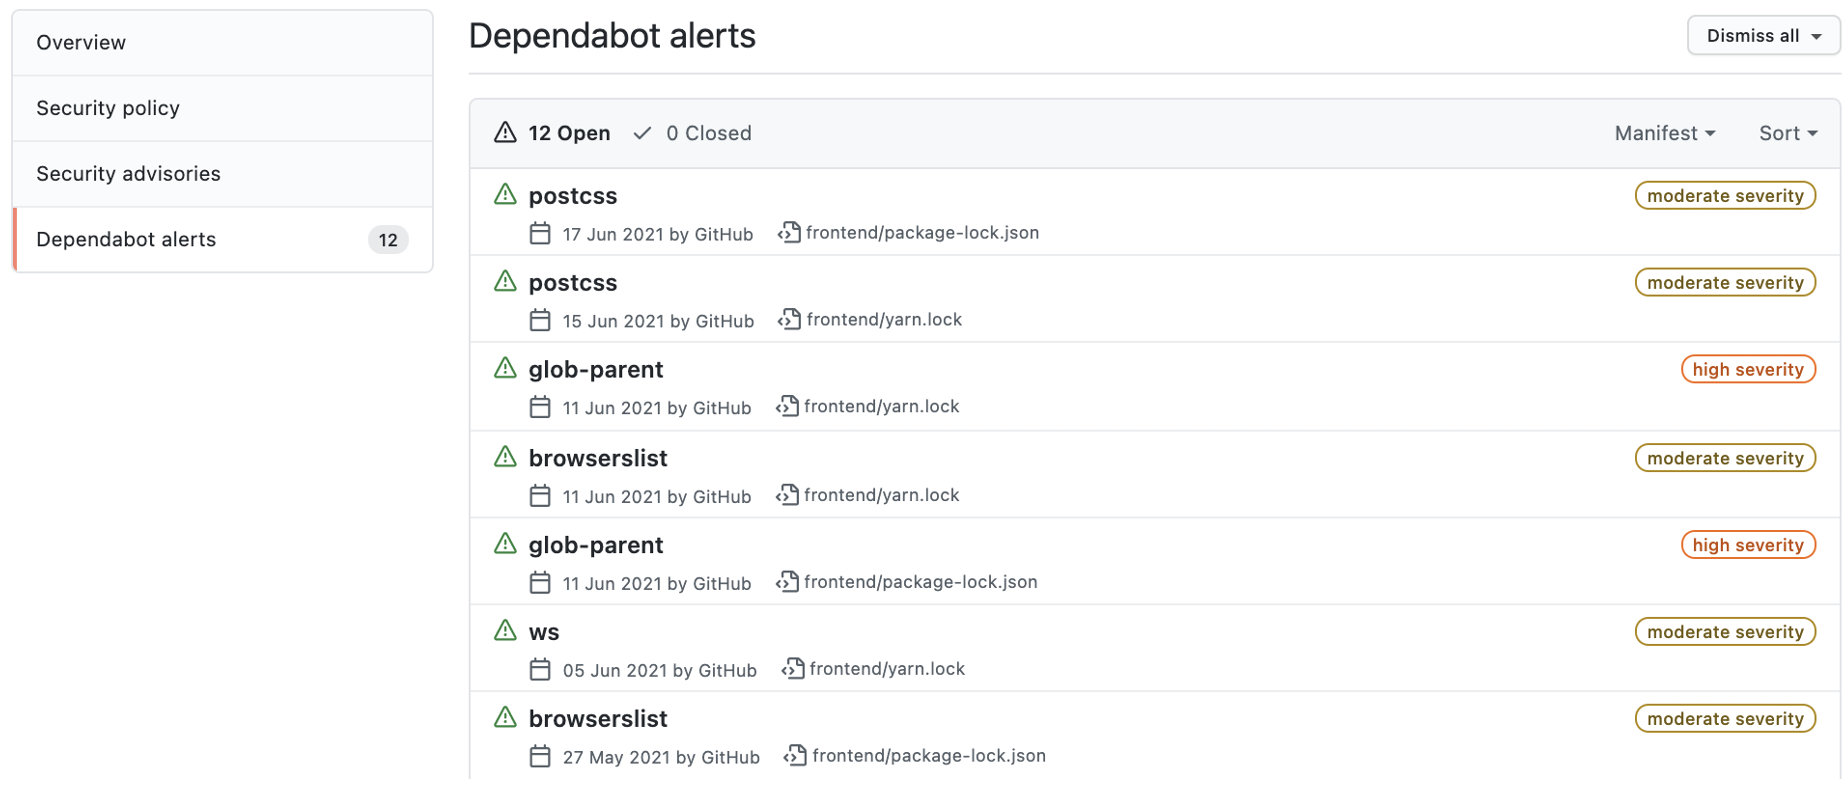
\includegraphics[width=1\textwidth]{images/dependabot.png}
  \caption{Dependabot alerts signalling library upgrades are required in the Atlas repository to prevent vulnerabilities.}
\end{figure}


\newpage

\section{Implementation}

\subsection{Local Artefact}
Atlas was made available as a local artefact on GitHub at https://github.com/jasminmartin/atlas. The application code was made open source. It is available to view, run or extend by members of the public. The GitHub repository is complete with documentation in the readme.md that advises users on how to run the application. The Latex report and images are contained within the repository along with instructions on how to generate the accompanying PDF.

\subsection{Deployment Strategy}
To release the application internally to the organisation, the author planned to host Atlas on the cloud. The cloud is a system of servers located in data centres all over the world (Pratim, 2018). The author had planned to release Atlas onto the Google Cloud Platform (GCP) as their organisation hosted the majority of their back-end applications on GCP. Before the application was deployed to GCP, the author would change the application architecture so that documents were stored in a Amazon S3 bucket (Figure X). This would ensure documents accessed by multiple members of the organisation would have consistent content. The back-end and front-end of Atlas would be hosted in separate Kubernetes pods in GCP. Both the front-end and back-end could be scaled individually to meet client load. Client requests would be directed with ingress that would enable access to the cluster.

\begin{figure}[!htb]
  \centering
      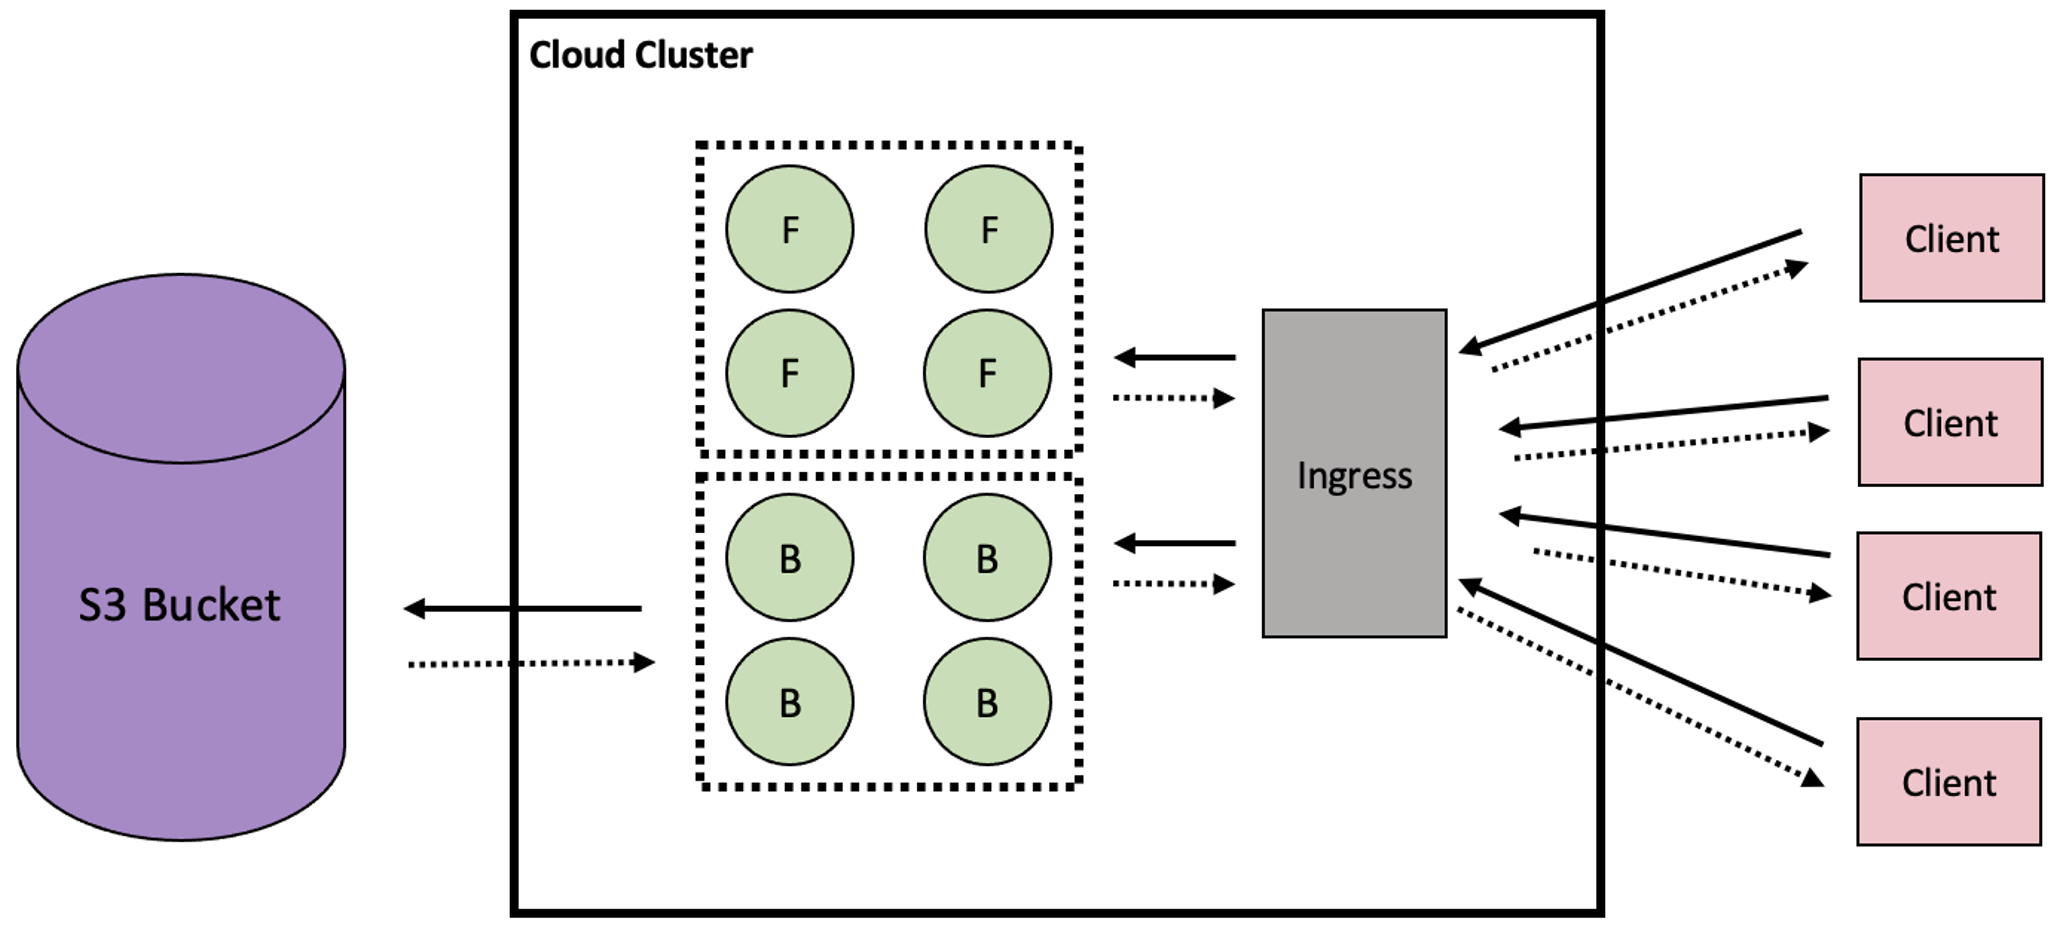
\includegraphics[width=1\textwidth]{images/deployment.png}
  \caption{Cloud-based architecture of Atlas. The green ‘F’ and ‘B’ circles represent the front-end and back-end pods.}
\end{figure}

To deploy new versions of Atlas to the cloud, the author would develop a continuous integration continuous deployment (CICD) pipeline. CICD pipelines automate the software delivery process by automatically building code, running tests and deploying to different environments. The former two processes were utilised in the development of Atlas using GitHub WorkFlows. In order to include continuous deployment into the pipeline, a more appropriate CICD pipeline solution could be used such as Jenkins. Jenkins extends the features of GitHub WorkFlow deploying the code into any number of gated environments. Each environment can test a different element of the service. For instance, an non-functional test environment may test the application passes load tests, whereas an integration environment can be used for developers to manually test features before they are released to production (Figure X).

\begin{figure}[!htb]
  \centering
      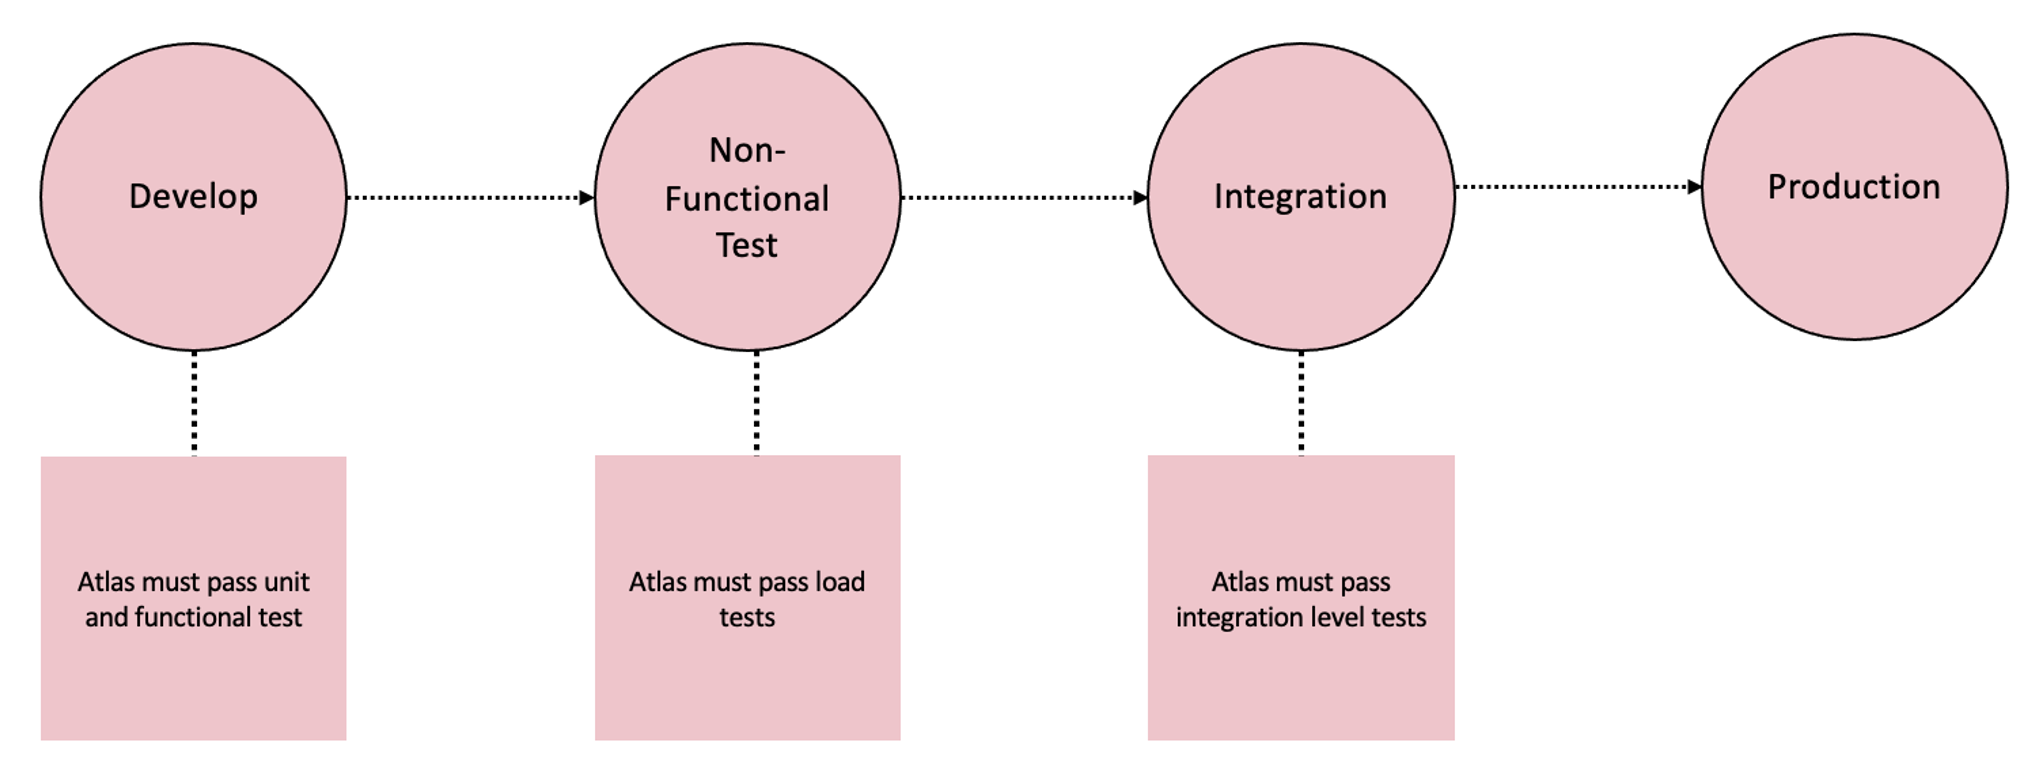
\includegraphics[width=1\textwidth]{images/jenkins.png}
  \caption{Jenkins pipeline setup could release the Atlas application into different environments.}
\end{figure}

\subsection{Metrics and Monitoring}

In order to provide a good level of service, it is important to maintain the performance and availability of a software application. Before Atlas is released into a production environment, the application must be able to generate and surface metrics. These metrics would be monitored to measure and alert the author of any problems with the user experience. Using the Kamon metrics instrumentation, the author could surface metrics that describe the traffic load, response time and response status codes (Kamon, 2021). These metrics could be visualised using a monitoring dashboard such as Grafana (Figure 27) (Grafana, 2021). Deviations of metrics above alerting thresholds could indicate problems with the infrastructure or application functionality. For instance, a high percentage of requests resulting in 404 status code responses could indicate a bug within the application. 

\begin{figure}[!htb]
  \centering
      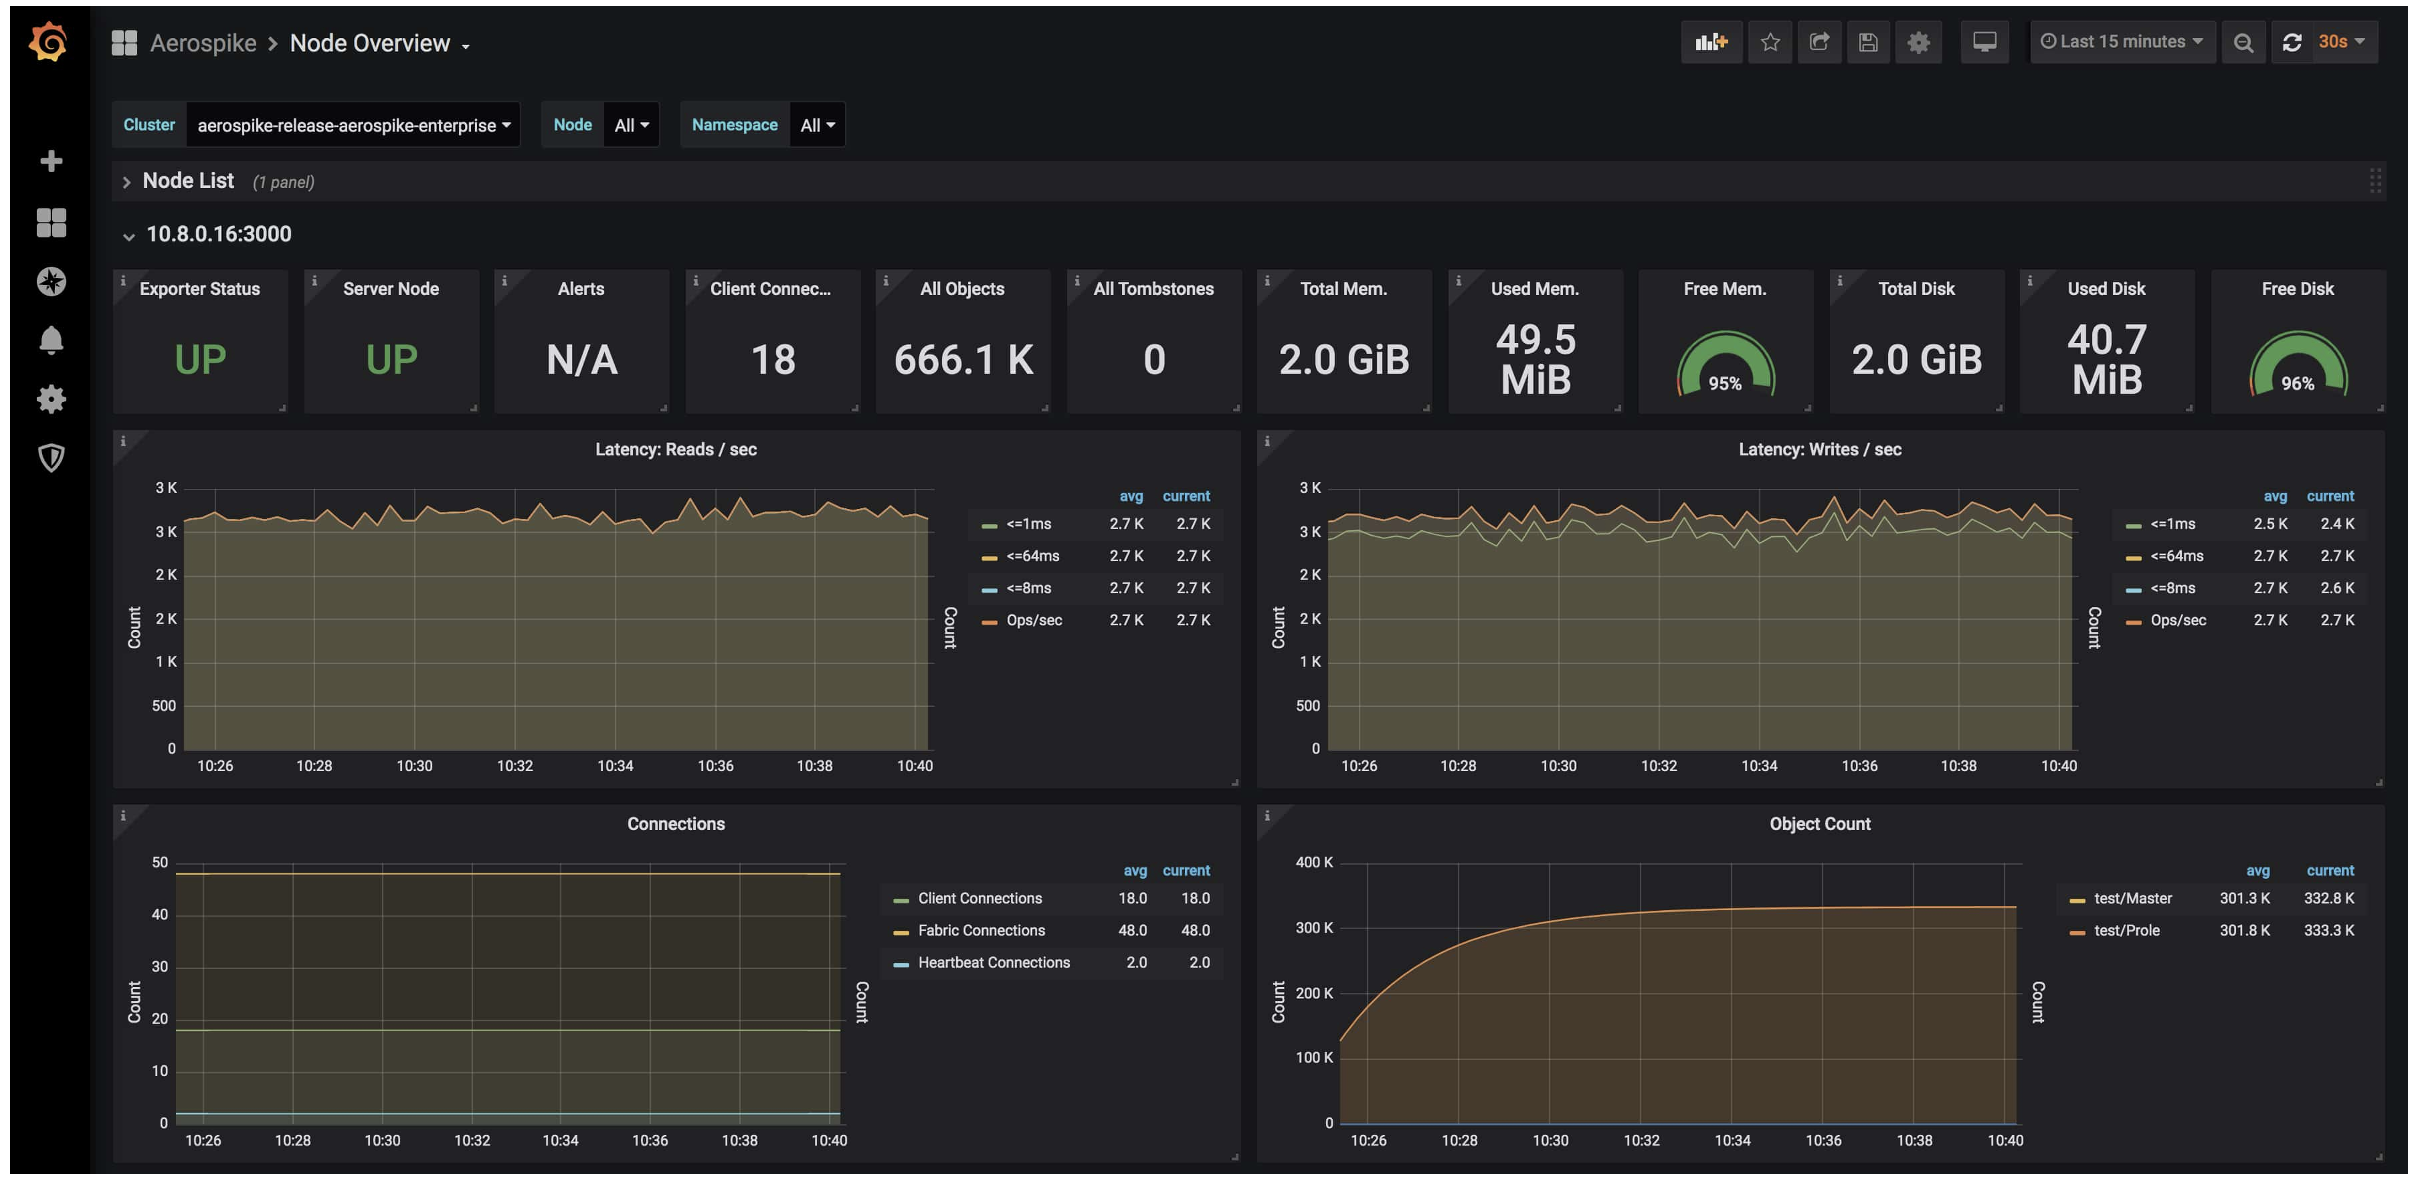
\includegraphics[width=1\textwidth]{images/grafana.png}
  \caption{An example of a Grafana monitoring dashboard (Pujari, 2019).}
\end{figure}

In addition to monitoring the API responses, it is also important to measure metrics related to computational resources usage. By understanding the CPU and memory usage of an application, the developer can predict the financial cost of running the application. Incorrect resource allocation could risk financial wastage or result in poor application performance (Pratim, 2018). Atlas would be deployed onto the Google Cloud Platform which provides an on-demand variability of computing resources. Although this means that pods can auto-scale to increase resource availability to meet load, it is still important to monitor resource usage as it may indicate issues with memory management in the application.

Once Atlas is released to customers, it is important to not only measure the performance of the application, but also the user experience. A common industry solution to measuring user experience is synthetic monitoring. Synthetic monitoring emulates the user journeys using scripts that mimic the user behaviour. It is important to measure the synthetic performance of the application to ensure customers have a positive user experience. Customer behaviour can be mimicked using technologies such a Dynatrace, which can be configured to perform common user journeys. Service level agreements outlining the expectations of the system are defined and the synthetic monitoring system will regularly test and alert if the application is not responding within the defined limits. An example of a service level agreement that could be tested is ‘a user will be able to view a newly added document within 750ms\textsuperscript{-1}’. The synthetic system will submit a new document, then click on the document when it appears on the Atlas web to view the content. If the sum of these requests is greater than 750ms\textsuperscript{-1}, the system will send an alert indicating a problem within this user journey.

\subsection{Further Functional Requirements}

As Atlas was developed using an agile management style, it would be possible to release the application in its current incrementation. However, future functional requirements could be added to Atlas to improve the user experience. The author did not full develop the automatic keyword suggestion feature (F8). As this ability would make the application unique from competing knowledge management tools, prioritising this feature could help the product stand out. To implement this feature, the author would build upon their knowledge of the Play framework which should be enable the application to efficiently store and list the common keywords that would be suggested.

To use the aforementioned deployment strategy (Figure X), Atlas would have to be modified so that it could maintain consistent content of shared documents (F11). This functionality would enable users in large organisations to easily update shared documents. As Atlas is currently configured to work with local file systems, the application would have to be integrated with an Amazon S3 bucket which would hold the state of the documents.

Although synthetic monitoring systems such as Dynatrace offer a thorough solution to monitoring user journeys, they require a subscription and maintenance cost. Whilst the customer base of Atlas is low, the author could implement a cheaper solution; collecting feedback via embedded in application surveys (F12). Such feedback could surface problems with the application usability, or uncover application bugs. Customer feedback widgets are one of the most common devices for gathering application feedback. Adding short survey in the context of the application offers a convenient way for customer to submit feedback. Such methods are proven to have higher response rates than email surveys (Spiess et al., 2012). 

\begin{table}[]
\centering
\small
\caption{Potential future functional requirements to be implemented into Atlas.}
\label{tab:my-table}
\resizebox{\textwidth}{!}{%
\begin{tabular}{|l|p{16cm}|}\hline
\textbf{No.} & \textbf{Functional Requirement} \\ \hline
\textbf{F8} & To automatically suggest new connections \\ \hline
\rowcolor[HTML]{FFCE93} 
\textbf{F11} & To maintain consistent shared documents \\ \hline
\rowcolor[HTML]{FFCE93} 
\textbf{F12} & To collect feedback via an embedded survey \\ \hline
\end{tabular}%
}
\end{table}

\newpage
\section{Conclusion}

The development  of Atlas provided the author with a mechanism for improving their project management and technical skills. Creating a greenfield application gave the author the opportunity to develop a product through the whole application life cycle; from soliciting requirements, to designing the user interface and experience. The author was guided through the development process with their chosen Scrumban Agile methodology. This project management style provided a framework for the author to iterate upon the application whilst gathering and incorporating user feedback. Throughout the process the author interacted and built relationships with different members of the department whilst building a tool which could aid the organisation. In total, the author achieved three of the four initial objectives, resulting in a functional iteration of Atlas.

Although the application was not deployed into a production environment, the resulting local artefact forms a strong basis which with further work, could be improve the comprehension of the organisations documentation. The project was successful as it exercised both the organisational and development skills of the author. In particular, the author improved their front-end development skills, as they became more confident using the React language. Furthermore, the author also learnt about natural language processing techniques, and formed a strong interest in working with big data manipulation in the future.

\newpage
\section{Further Work}

For Atlas to be used in an organisational setting, it must be deployed into a production environment. The previously described deployment strategy could be executed within the next 8 week development period (Figure 28). A small functional change to the document storage would first enable the cloud-based deployment. The author would also implement metrics and monitoring to ensure the application is running smoothly in production. The authors organisation already has Jenkins pipeline infrastructure and GCP environments configured, so the author estimates it would only take a further 4 weeks of development to deploy Atlas into production. The author would prioritise the automatic tag recommendation as the next developed feature as they have already researched into big data processing strategies.

\begin{figure}[!htb]
  \centering
      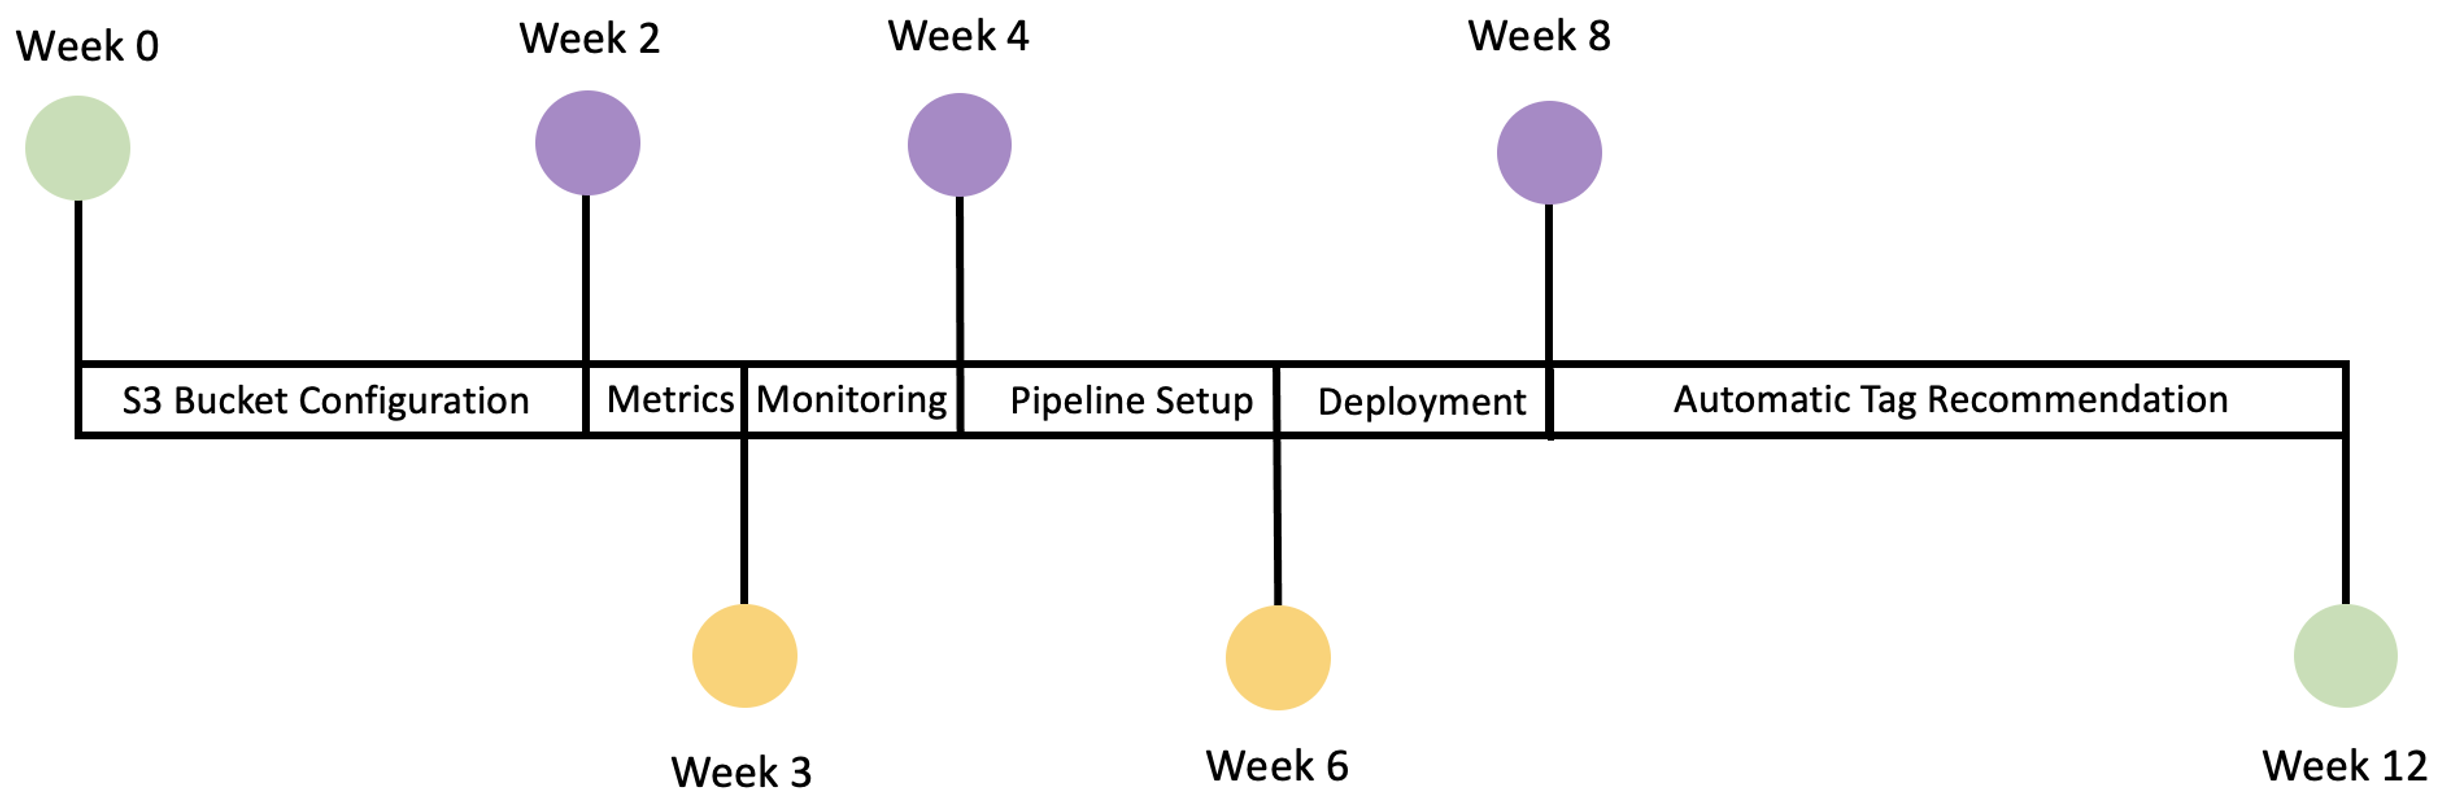
\includegraphics[width=1\textwidth]{images/future-timeline.png}
  \caption{The author would dedicate the next 8 weeks of development to ensuring Atlas was ready to be deployed into production. A further estimated 4 weeks could then be used to develop the automatic tag recommendation feature.}
\end{figure}

In addition to developing the application functionality and infrastructure further, the author would also dedicate effort to introducing more developers in the organisation to Atlas. As the product will remain with the organisation, it is important to future-proof the application by ensuring other developer have context on the application code and understand the related documentation. The author could engage more developers into the project by demoing the deployed product in the department showcase and encouraging audience members to take part in the next stages of development.

\newpage
\section{Reflective Statement}


\newpage
\section{Glossary}
{\parindent0pt
\textbf{Agile}: A software development methodology focused on iterative cycles of development. Requirements and results are continuously evaluated to quickly respond to change.

\textbf{API}: Application Programming Interface is a software intermediary that enables two applications to communicate with each other.

\textbf{Atlas Web}: The main user interface of the Atlas application that displays the file system as a graph.

\textbf{Cloud Programming}: An on-demand availability of computer system resources and data storage, that does not require direct active management. 

\textbf{Cluster}: A shared group of networking resources for kubernetes pods.

\textbf{CORS}: Cross-Origin Resource Sharing is an HTTP-header based mechanism that secures browsers by limiting the domains and ports from which resources can be received.

\textbf{Docker}: a containerized platform that combines the application source code, libraries and operating system into a specific environment.

\textbf{Extreme Programming}: A software development methodology focused upon improving software quality and the speed of response to changing customer requirements.

\textbf{GCP}: Google Cloud Platform is a provider of cloud computing resources for developing, deploying, and operating software applications.

\textbf{Github}: A website that hosts software and acts as a version control system.

\textbf{Jenkins}: An automation pipeline which enables software to be built, tested, and deployed into different environments.

\textbf{Kanban}: An agile workflow management method for defining, managing and improving software development.

\textbf{Kubernetes}: A container-orchestration system for automatically deploying, scaling, and managing applications in pods.

\textbf{Pod}: Point of delivery, is a module of application components, storage and network resources that work together to deliver a service.

\textbf{S3 Bucket}:  a cloud storage system that utilises in Amazon Web Services' (AWS). Also known as the Simple Storage Service.

\textbf{Scrum}: An agile framework for developing and delivering products, by generating adaptive solutions that help organise teams and organisations.

\textbf{Scrumban}: An agile development methodology that is a hybrid of Scrum and Kanban.

\textbf{Spike}: An extreme programming practice whereby a developer allocates a time period to research or prototype a technical solution.

\textbf{Transitive Dependency}: A software dependency that is introduced by the libraries that the program references.
}
\newpage
\section{References}
{\parindent0pt
Abraham, A., 2021. Cheatsheet Differences Scrum vs Scrumban vs Kanban. [online] Medium. Available at: $<$ \url{https://medium.com/agileinsider/comparison-of-scrum-vs-scrumban-vs-kanban-1d1d2b9a9fd5}$>$ [Accessed 3 October 2021].

Afzal, Wasif, Richard Torkar, and Robert Feldt. "A systematic review of search-based testing for non-functional system properties." Information and Software Technology 51, no. 6 (2009): 957-976.

Agiledictionary.com. 2021. Spike | The Agile Dictionary. [online] Available at: $<$ \url{http://agiledictionary.com/209/spike/}$>$ [Accessed 3 October 2021].

Anthony I. Wasserman. 2010. Software engineering issues for mobile application development. In Proceedings of the FSE/SDP workshop on Future of software engineering research. Association for Computing Machinery, New York, NY, USA, pp.397–400. 

Asra Khalid, Sobia Zahra, Muhammad Fahad Khan. 2014. Suitability and Contribution of Agile Methods in Mobile Software Development, IJMECS, 6(2) pp.56-62.

Augustine, S., Payne, B., Sencindiver, F., Woodcock, S. 2005. Agile project management: Steering from the edges. ACM. 48 pp.85-89.

Beck, K. 2003. Test-driven development: by example. Addison-Wesley Professional.

Chowdhury, G. 2005. Natural language processing. ARIST. 37 pp.51-89. 

Clark, K. 2021. A \$200 Million Seed Valuation for Roam Shows Investor Frenzy for Note-Taking Apps. [online] The Information. Available at: $<$ \url{https://www.theinformation.com/articles/a-200-million-seed-valuation-for-roam-shows-investor-frenzy-for-note-taking-apps?shared=931cbf4ce58ed9bd}$>$ [Accessed 3 October 2021].

Coleman, J., McTigue, E. and Dantzler, J., 2018. What Makes a Diagram Easy or Hard? The Impact of Diagram Design on Fourth-Grade Students’ Comprehension of Science Texts. The Elementary School Journal. 119(1) pp.122-151.

Damerau, F. and Indurkhya, N., 2010. Handbook of natural language processing. Boca Raton, Estados Unidos: Taylor & Francis. 2 pp.72-78.

Dawson, C. 2015. Projects in Computing and Information Systems. Harlow, United Kingdom: Pearson Education, Limited.

Developer.mozilla.org. 2021. Cross-Origin Resource Sharing (CORS) - HTTP | MDN. [online] Available at: $<$ \url{https://developer.mozilla.org/en-US/docs/Web/HTTP/CORS}$>$ [Accessed 3 October 2021].

Distroless Docker: Containerizing Apps, not VMs. 2017. [video] Directed by M. Moore. Napa, California: swampUP 2017.

Doherty, N., Champion, D. and Wang, L. 2010. An holistic approach to understanding the changing nature of organisational structure. Information Technology & People, 23(2), pp.116-135.

Dybå T., Dingsøyr T., Moe N.B. 2014. Agile Project Management. In: Ruhe G., Wohlin C. Software Project Management in a Changing World. Springer, Berlin, Heidelberg.

Eliason, N. 2020. Roam: Why I Love it and How I use it. Nateliason. Available at: $<$ \url{https://www.nateliason.com/blog/roam }$>$ [Accessed 1 October 2021].

Forte, T. 2021. How To Take Smart Notes: 10 Principles to Revolutionize Your Note-Taking and Writing - Forte Labs. [online] Forte Labs. Available at: $<$ \url{https://fortelabs.co/blog/how-to-take-smart-notes/?fbclid=IwAR0Dbtdio3oYPicwAaFToU1EiEBrXGiQavUxv8lR2CSMaupAKQASeT-Ckts}$>$ [Accessed 14 May 2021].

Fowler, M. 2003. UML Distilled: A Brief Guide to the Standard Object Modeling. 2nd ed. Addison Wesley, pp.32-45.

Fowler, M.,  Highsmith, J. 2000. The Agile Manifesto.

Ghemawat, S., Gobioff, H. and Leung, S, 2003. The Google file system. ACM SIGOPS Operating Systems Review, 37(5), pp.29-43.

Gibbs, A., 1997. Focus groups. Social research update, 19(8), pp.1-8.

Gibson, B., 2021. Building a Slip-Box. Available at: $<$ \url{https://www.barryjohngibson.com/post/down-the-rabbit-hole-building-a-slip-box-or-zettelkasten}$>$ [Accessed 14 May 2021].

GitHub. 2021. Dagrejs/dagre. [online] Available at: $<$ \url{https://github.com/dagrejs/}$>$ [Accessed 3 October 2021].

Grafana.com. 2021. [online] Available at: $<$ \url{https://grafana.com/}$>$ [Accessed 3 October 2021].

Gunwoong L., Raghu T. 2014 Determinants of Mobile Apps' Success: Evidence from the App Store Market, Journal of Management Information Systems, 31(2), pp.133-170.

Hegarty, M., Carpenter, P. A., Just, M. A. 1991. Diagrams in the comprehension of scientific texts. Handbook of reading research, 2 pp.641–668.

Hoda, R., Noble, J., Marshall, S., 2008. Agile project management. In New Zealand Computer Science Research Student Conference, NZCSRC.

Jeffries, R. 2021. RonJeffries.com. [online] Available at: $<$ \url{https://ronjeffries.com/}$>$ [Accessed 3 October 2021].

Jivani, A.G. 2011. A comparative study of stemming algorithms. International Journal of Computer Technology, 2(6), pp.1930-1938.

Johnson-Laird, P. N. 1983. Mental Models : Towards a Cognitive Science of Language, Inference, and Consciousness. Cambridge University Press. pp. 3-18.

Juristo, N. and Vegas, S. 2003. Functional testing, structural testing and code reading: What fault type do they each detect?. Empirical Methods and Studies in Software Engineering. pp. 208-232. 

Springer, T., Berlin, K., Heidelberg., O. Kamon.io. 2021. Performance Monitoring Tools for Backend Services and APIs. [online] Available at: $<$ \url{https://kamon.io/}$>$ [Accessed 3 October 2021].

Liddy, E. 2001. Natural Language Processing. Information Processing & Management, 26(1), pp.39-52.

Lidwell, W., Holden, K., Elam, K. and Butler, J. 2003. Universal principles of design. Beverly, Mass: Rockport Publishers. pp. 32-54

Lüdecke, D. 2015. Introduction into Luhmanns Zettelkasten-Thinking and its Technical Implementation. Cognitive Science. 2(3) pp. 2-4.

Martin, JF. 2020. My Review of Notion from a Bloggers Perspective. Numeric Citizen. Available at: https://numericcitizen.me/2020/04/19/my-review-of-notion-from-a-bloggers-perspective/

Nilsson, N.J. 2014. Principles of artificial intelligence.

nvd.nist.gov. 2021. NVD - CVE-2010-4051. [online] Available at: $<$ \url{https://nvd.nist.gov/vuln/detail/CVE-2010-4051}$>$ [Accessed 3 October 2021].

nvd.nist.gov. 2021. NVD - CVE-2021-2388. [online] Available at: $<$ \url{https://nvd.nist.gov/vuln/detail/CVE-2021-2388}$>$ [Accessed 3 October 2021].

Partha-Partim, R. 2018. An Introduction to Dew Computing: Definition, Concept and Implications - IEEE Journals and Magazine. IEEE Access. 6 pp.723–737. 

Playframework.com. 2021. Play Framework - Build Modern & Scalable Web Apps with Java and Scala. [online] Available at: $<$ \url{https://www.playframework.com/}$>$ [Accessed 3 October 2021].

Pujari, S., 2021. JMeter Grafana Dashboard using InfluxDB - Step-by-step Guide. [online] PerfMatrix. Available at: $<$ \url{https://www.perfmatrix.com/jmeter-grafana-dashboard-using-influxdb/}$>$ [Accessed 3 October 2021].

Rana, A., Gautam, S., Mann, P. and Tyagi, N. 2020. Classification for Big Data Tools and Its Challenges and Issues. SSRN Electronic Journal. pp. 32-41

Reardon, D. 2004. Doing an undergraduate project. 1st ed. London: SAGE.

Reis, E., 2009. Minimal Viable Produce: a Guide. [online] Available at:  $<$ {\url{http://www.startuplessonslearned.com/2009/08/minimum-viable-product-guide.html}}$>$ [Accessed 25 June 2021].

Roam Research. 2021. Roam Research – A note taking tool for networked thought.. [online] Available at: $<$ \url{https://roamresearch.com/}$>$ [Accessed 3 October 2021].

Roestenburg, R., Bakker, R., and Williams. 2016. Akka in Action. Manning.

Roper, J, 2012. Benchmarking Scala against Java. [online] Available at:  $<$ \url{https://dzone.com/articles/benchmarking-scala-against}$>$ [Accessed 4 June 2021].

Samhi, J., Allix, K., Bissyandé, T.F. 2021. A first look at Android applications in Google Play related to COVID-19. Empire Software Engineering. 26 pp.57.

Scheiter, K., Eitel, A. 2015. Signals foster multimedia learning by supporting integration of highlighted text and diagram elements. Learning and Instruction. 36, pp.11-26.

Schiller, M., Sönke, A. 2017. How to Take Smart Notes: One Simple Technique to Boost Writing, Learning and Thinking for Students, Academics and Nonfiction Book Writers. Journal of Writing Research , 9(2), pp.227-231.

Spiess, J., T'Joens, Y., Dragnea, R., Spencer, P. and Philippart, L. 2014. Using big data to improve customer experience and business performance. Bell labs technical journal, 18(4), pp.3-17.

Stellman, A. and Greene, J., 2008. Applied software project management. Sebastopol, CA: O'Reilly.

Stellman, A. and Greene, J., 2008. Applied software project management. Sebastopol, CA: O'Reilly.

Stone, D., Jarrett, C., Woodroffe, M. and Minocha, S., 2005. User Interface Design and Evaluation. Amsterdam: Elsevier, pp.1-30.

Trujillo, S. 2018. How To Parse Hashtags and Mentions with a Tokenizer in NodeJS. [online] Medium. Available at: $<$ \url{https://medium.com/@sonny.io/how-to-parse-hashtags-and-mentions-with-a-tokenizer-in-nodejs-e7756730b573}$>$ [Accessed 21 May 2021].

Turing, M, A. 1950. Computing and Machinery Intelligence. 236, pp.433-460.

Ventsislav, Y. 2018. Introduction to Natural Language Processing for Text. [online] Medium. Available at: $<$ \url{https://towardsdatascience.com/introduction-to-natural-language-processing-for-text-df845750fb63}$>$ [Accessed 21 May 2021].
}

\newpage
\section{Appendix 1}
{\parindent0pt
\subsection{Survey Questions}
1. What is your job role? (Open question)

2. How much do you feel like you understand what the product is trying to achieve? (1-10)

3. If available, how likely would you be to use the product when understanding documentation? (1-10)

4. How clear do you think the graph view user interface is? (Included Photo of user interface) (1-10)

5. Is there anything in particular you would like to see improved to the net view user interface? (Open question)

6. How clear do you think the user journey is? (1-10)

7. Which feature would you like to see next? (Order options)
- Lemmatization (included definition)
- Show sub-graphs
- Delete notes
- Add new notes
- Open documents

8. Are there any additional features that you would like to see implemented in Zettelkasten? (Open question)

9. Any additional comments regarding Zettelkasten? (Open question)

\subsection{Focus Group Notes}
U2,U3,U6 - confusion how web relates to file system

U1 - suggested instruction guide

U2 - suggested video

General preference of instruction guide

All users - dislike the size of web, too big / complex

Author suggests zoom feature - 5 users agree

U4 - wants AI tag suggestion feature, all users agree

U5 - dislikes name of product, too confusing. Other users agree
}
\end{document}